\documentclass[12pt,a4paper]{report}

\usepackage[T1]{fontenc}
\usepackage{mathptmx} % Times New Roman for text and math
\usepackage{graphicx}
\usepackage{ragged2e}
\usepackage{geometry}
\usepackage{setspace}
\usepackage{fancyhdr}
\usepackage{xcolor}
\usepackage{longtable}
\usepackage{array}
\usepackage{booktabs}
\usepackage{enumitem}
\usepackage{hyperref}
\usepackage{float}
\usepackage{tocloft}
\usepackage[justification=centering]{caption}
\usepackage{multirow}
\usepackage{amsmath}
\usepackage{titlesec}
\usepackage{chngcntr}
\usepackage{etoolbox}

%---------------------------------------------
% Margins
%---------------------------------------------
\geometry{
left=1in,
right=1in,
top=1in,
bottom=1in
}

\setstretch{1.5}

%---------------------------------------------
% Figure / Table numbering per chapter (e.g. Fig 3.2, Table 3.2)
%---------------------------------------------
\counterwithin{figure}{chapter}
\counterwithin{table}{chapter}

%---------------------------------------------
% Caption style: Times New Roman size 10
% Figure caption BELOW figure, Table caption ABOVE table
%---------------------------------------------
\captionsetup[figure]{font=small,labelfont=bf,position=bottom}
\captionsetup[table]{font=small,labelfont=bf,position=top}

%---------------------------------------------
% Chapter Title: 16pt Bold, ALL CAPS, Centered
% Side Headings (Section): 12pt Bold, ALL CAPS
% Subsection: 12pt Bold
%---------------------------------------------
\titleformat{\chapter}[block]
  {\centering\fontsize{16}{19}\bfseries}
  {\MakeUppercase{\chaptertitlename} \thechapter :}
  {0.5em}
  {\MakeUppercase}

\titlespacing*{\chapter}{0pt}{-10pt}{20pt}

\titleformat{\section}
  {\fontsize{12}{14}\bfseries}
  {\thesection}
  {0.6em}
  {\MakeUppercase}

\titleformat{\subsection}
  {\fontsize{12}{14}\bfseries}
  {\thesubsection}
  {0.6em}
  {}

\titleformat{\subsubsection}
  {\fontsize{12}{14}\bfseries\itshape}
  {\thesubsubsection}
  {0.6em}
  {}

%---------------------------------------------
% Avoid a page ending with a heading, or a single
% orphan/widow line of a new paragraph
%---------------------------------------------
\clubpenalty=10000
\widowpenalty=10000
\displaywidowpenalty=10000
\raggedbottom

%---------------------------------------------
% Header / Footer style
% Header: Project Name (left) + Page number (right), dark red, size 10, with rule
% Footer: Department name, size 10, with rule
%---------------------------------------------
\definecolor{darkred}{RGB}{139,0,0}

\pagestyle{fancy}
\fancyhf{}
\renewcommand{\headrulewidth}{0.8pt}
\renewcommand{\footrulewidth}{0.8pt}
\patchcmd{\headrule}{\hrule}{\color{darkred}\hrule}{}{}
\patchcmd{\footrule}{\hrule}{\color{darkred}\hrule}{}{}

\fancyhead[L]{\small\textbf{AeroCrew}}
\fancyhead[R]{\small\thepage}
\fancyfoot[L]{\small Department of Computer Science, CHRIST (Deemed to be University)}

% Style used for chapter opening pages (fancy still applies, but no header rule text change needed)
\fancypagestyle{plain}{%
  \fancyhf{}
  \renewcommand{\headrulewidth}{0.8pt}
  \renewcommand{\footrulewidth}{0.8pt}
  \patchcmd{\headrule}{\hrule}{\color{darkred}\hrule}{}{}
  \patchcmd{\footrule}{\hrule}{\color{darkred}\hrule}{}{}
  \fancyhead[L]{\small\textbf{AeroCrew}}
  \fancyhead[R]{\small\thepage}
  \fancyfoot[L]{\small Department of Computer Science, CHRIST (Deemed to be University)}
}

% Style for pages with NO header/footer (Title Page, Certificate, TOC)
\fancypagestyle{empty}{%
  \fancyhf{}
  \renewcommand{\headrulewidth}{0pt}
  \renewcommand{\footrulewidth}{0pt}
}

\begin{document}

\normalfont
\fontsize{12}{18}\selectfont

%%%%%%%%%%%%%%%%%%%%%%%%%%%%%%%%%%%%%
% TITLE PAGE  -- no header/footer
%%%%%%%%%%%%%%%%%%%%%%%%%%%%%%%%%%%%%

\begin{titlepage}
\thispagestyle{empty}

\begin{center}


\includegraphics[width=0.65\textwidth]{logo.png}

\vspace{1.5cm}

{\fontsize{16}{19}\selectfont 
\textbf{AEROCREW: INTELLIGENT AIRLINE MANAGEMENT AND DISRUPTION RECOVERY DECISION SUPPORT SYSTEM}
}

\vspace{0.5cm}

{\fontsize{13}{16}\selectfont \textbf{By}}

\vspace{0.5cm}

{\fontsize{14}{18}\selectfont
Jiya Elza Jabi (2547123) \\
Shalwin Biju (2547150) \\
Shubham Swaraj (2547155)
}

\vspace{1.5cm}

{\fontsize{13}{16}\selectfont Under the guidance of}

\vspace{0.2cm}

{\fontsize{14}{18}\selectfont \textbf{Dr. Kavitha R}}

\vspace{1.5cm}

{\fontsize{13}{17}\selectfont
Specialization Project report submitted in partial fulfilment of the requirements of IV Trimester MCA,\\
CHRIST (Deemed to be University)
}

\vspace{0.8cm}

{\fontsize{13}{16}\selectfont August -- 2026}

\end{center}

\end{titlepage}

%%%%%%%%%%%%%%%%%%%%%%%%%%%%%%%%%%%%%
% CERTIFICATE PAGE -- no header/footer
%%%%%%%%%%%%%%%%%%%%%%%%%%%%%%%%%%%%%

\begin{titlepage}
\thispagestyle{empty}

\begin{center}


\includegraphics[width=0.65\textwidth]{logo.png}

\vspace{1cm}

{\fontsize{16}{19}\selectfont \textbf{CERTIFICATE}}

\vspace{1cm}
\begin{justify}
\textit{
This is to certify that the report titled \textbf{AeroCrew: Intelligent Airline Management and Disruption Recovery Decision Support System}  is a bona fide record of work done by Jiya Elza Jabi (2547123), Shalwin Biju(2547150) and Shubham Swaraj(2547155) of CHRIST (Deemed to be University), Bangalore, in partial fulfilment of the requirements of IV Trimester MCA during the year 2026
}
\end{justify}
\vspace{0.5cm}



\noindent
\begin{tabular}{@{}p{7cm} p{7cm}@{}}
\textbf{Head of the Department} &
\textbf{Project Guide}
\end{tabular}

\vspace{1.5cm}

\noindent
\begin{tabular}{@{}p{5cm} p{9cm}@{}}

\textbf{Valued by:} & \\[0.8cm]

1. & Name \hspace{2.7cm}: Shalwin Biju \\[0.4cm]

2. & Register Number \hspace{0.85cm}: 2547150\\[0.4cm]

& Examination Centre \hspace{0.45cm}: CHRIST (Deemed to be University) \\[0.4cm]

& Date of Exam \hspace{1.45cm}: \\

\end{tabular}

\end{center}

\end{titlepage}

%---------------------------------------------
% AI USAGE DECLARATION
%---------------------------------------------

\begin{titlepage}
\thispagestyle{plain}
\pagenumbering{roman}
\setcounter{page}{3}
\pagestyle{plain}

\begin{center}
{\fontsize{15}{18}\selectfont \textbf{AI USAGE DECLARATION STATEMENT}}
\end{center}

\vspace{0.2cm}

{\fontsize{11}{14}\selectfont
\begin{justify}

I hereby declare that Artificial Intelligence tools were used only for supportive purposes such as idea exploration, conceptual understanding, literature guidance, and grammar refinement during the development of this project. No AI generated code has been copied or submitted, and all programming, model development, experimentation, analysis, and results were independently developed and implemented by me or our team. I confirm that this project is our original work and reflects our own understanding and effort, and I take full responsibility for its authenticity and adherence to academic integrity policies.

\vspace{0.25cm}

I also declare that the approximate usage of Artificial Intelligence tools for supportive purposes in this project is 20\%, limited to idea exploration, literature search guidance, grammar refinement, clarification of technical concepts, and other academic assistance.

\vspace{0.25cm}

The details of AI tools used in this project and their purpose are listed below:

\vspace{0.1cm}

\begin{enumerate}[leftmargin=0.6cm,itemsep=0.15cm]

\item \textbf{Name of the AI Tool:} ChatGPT (OpenAI)\\
\textbf{Purpose of Use:} Code debugging, algorithm development

\item \textbf{Name of the AI Tool:} Google Gemini\\
\textbf{Purpose of Use:} Research assistance

\item \textbf{Name of the AI Tool:} Claude (Anthropic)\\
\textbf{Purpose of Use:} Project report writing, documentation formatting

\end{enumerate}

\vspace{0.1cm}

This declaration confirms that the AI tools mentioned above were used only for supportive and assistive purposes and that no AI generated code has been directly copied or submitted as part of this project.

\end{justify}
}

\vspace{0.1cm}

\begin{flushleft}

\begin{tabular}{@{}p{5cm} c p{8cm}@{}}

\textbf{Name of the Student} & : & Shalwin Biju \\[0.4cm]

\textbf{Register Number} & : & 2547150 \\[0.4cm]

\textbf{Project Title} & : & AeroCrew: Intelligent Airline Management and Disruption Recovery Decision Support System \\[0.5cm]

\textbf{Signature} & : & \\[0.4cm]

\textbf{Date} & : & \\

\end{tabular}

\end{flushleft}

\end{titlepage}

%%%%%%%%%%%%%%%%%%%%%%%%%%%%%%%%%%%%%
% FRONT MATTER -- lower case roman numerals
% starting from Acknowledgements
%%%%%%%%%%%%%%%%%%%%%%%%%%%%%%%%%%%%%


\pagenumbering{roman}
\setcounter{page}{4}
\pagestyle{plain}
\chapter*{ACKNOWLEDGEMENT}
\addcontentsline{toc}{chapter}{ACKNOWLEDGEMENT}

We would like to express our sincere gratitude to all those who supported and guided us throughout the development of this project.\\ 
First and foremost, we would like to thank Fr. Jossy P George, Director of CHRIST (Deemed to be University), for the visionary leadership and for providing an environment that encourages academic excellence and research.\\
We also extend our heartfelt thanks to Dr. Rupali Sunil Wagh, Head of the Department of Computer Science, and Dr. Gobi R, Associate Head of the Department of Computer Science, for providing us with the opportunity and the necessary facilities to carry out this project successfully.\\
We would like to express our sincere appreciation to Dr. Cynthia T, the Program Coordinator for MCA and MSc AIML, for the constant support, coordination, and encouragement throughout the duration of this project.\\
We would also like to express our special thanks to our project guide, Dr. Kavitha R, for the valuable guidance, continuous support, insightful suggestions, and constructive feedback offered during the entire course of this project.\\
We are also thankful to all the faculty members of the department for sharing their knowledge and providing the academic support required for completing this project.\\ 
Finally, we would like to thank our friends and family members for their encouragement, understanding, and support throughout the process of completing this project.


\newpage

%%%%%%%%%%%%%%%%%%%%%%%%%%%%%%%%%%%%%
% ABSTRACT (single spaced, <=200 words, no sub-heads/bullets)
%%%%%%%%%%%%%%%%%%%%%%%%%%%%%%%%%%%%%

\chapter*{ABSTRACT}
\addcontentsline{toc}{chapter}{ABSTRACT}


The aviation industry operates in an environment where operational efficiency, safety, and regulatory compliance are critical for ensuring uninterrupted flight operations. One of the major challenges faced by airline Operations Control Centers (OCCs) is managing unexpected crew disruptions caused by pilot illness, duty-time violations, weather conditions, or unforeseen operational constraints. Manual crew recovery processes are often time consuming, error-prone, and unable to respond efficiently under strict operational deadlines. \\
AeroCrew is an intelligent airline crew management and disruption recovery decision support system designed to automate and optimize the crew recovery process. The system continuously monitors operational data, validates pilot eligibility according to Directorate General of Civil Aviation (DGCA) Flight Duty Time Limitation regulations, estimates travel time to departure airports, and ranks eligible standby pilots using a rule-based decision engine. Rather than replacing human decision making, the platform provides explainable recommendations that assist Operations Controllers in selecting the most suitable replacement pilot while maintaining complete operational transparency.\\
The application follows a modern three-tier architecture consisting of a React based web dashboard, a Spring Boot REST backend, PostgreSQL database, and an Android mobile application for pilots. The modular architecture enables scalability, maintainability, security, and future integration with external airline systems. \\
The proposed solution minimizes flight delays, improves operational efficiency, reduces regulatory risks, enhances crew utilization, and provides a centralized platform for intelligent airline crew management. The system demonstrates how Artificial Intelligence assisted decision support can significantly improve airline operational resilience while maintaining human oversight over critical decisions.



\newpage

%%%%%%%%%%%%%%%%%%%%%%%%%%%%%%%%%%%%%
% TABLE OF CONTENTS -- no header/footer, no page number
%%%%%%%%%%%%%%%%%%%%%%%%%%%%%%%%%%%%%

\thispagestyle{empty}
\tableofcontents
\clearpage

\thispagestyle{empty}
\listoffigures
\clearpage

\thispagestyle{empty}
\listoftables
\clearpage

%%%%%%%%%%%%%%%%%%%%%%%%%%%%%%%%%%%%%
% MAIN MATTER -- Arabic numbering starts at Chapter 1
%%%%%%%%%%%%%%%%%%%%%%%%%%%%%%%%%%%%%

\pagestyle{fancy}
\pagenumbering{arabic}
\setcounter{page}{1}

%%%%%%%%%%%%%%%%%%%%%%%%%%%%%%%%%%%%%
% CHAPTER 1
%%%%%%%%%%%%%%%%%%%%%%%%%%%%%%%%%%%%%

\chapter{INTRODUCTION}

Modern airline operations rely on accurate crew scheduling, regulatory compliance, and rapid decision making to ensure uninterrupted flight operations. This chapter introduces the background, objectives, scope, applicability, and overall purpose of the AeroCrew AI system while providing an overview of the report.

\section{BACKGROUND OF THE PROJECT}

The aviation industry has experienced rapid technological transformation over the past decade, with airlines increasingly adopting intelligent software systems to improve operational efficiency and passenger satisfaction. One of the most complex operational activities performed within an airline Operations Control Center (OCC) is managing airline crew assignments. Every commercial flight requires qualified crew members who satisfy licensing, medical fitness, aircraft rating, and Flight Duty Time Limitation (FDTL) regulations established by aviation authorities.

Crew disruptions may occur unexpectedly because of illness, personal emergencies, weather conditions, delayed inbound flights, technical failures, airport congestion, or duty-hour violations. In such situations, airline controllers must quickly identify an eligible replacement pilot while ensuring compliance with regulatory policies and minimizing flight delays. Traditional manual recovery procedures involve multiple software systems, spreadsheets, telephone communication, and extensive human verification, making the process slow and highly susceptible to human error.

AeroCrew AI is proposed as an intelligent decision support platform that integrates crew management, compliance verification, disruption recovery, candidate ranking, operational dashboards, and mobile notifications into a unified software solution. The system assists airline controllers by automatically identifying qualified standby pilots based on regulatory compliance, operational constraints, geographical proximity, estimated travel time, and pilot availability. Instead of replacing human expertise, the platform augments decision making through explainable recommendations supported by real-time operational data.

Furthermore, the project contributes towards the United Nations Sustainable Development Goal (SDG 9 -- Industry, Innovation and Infrastructure) by promoting innovation in aviation technology and improving the resilience of transportation infrastructure through intelligent automation.

\section{OBJECTIVES}

The primary objective of AeroCrew AI is to develop an intelligent airline crew management and disruption recovery platform capable of assisting Operations Control Center (OCC) personnel in making accurate, timely, and regulation-compliant crew assignment decisions. The system combines real-time operational monitoring, compliance validation, automated candidate ranking, and centralized management into a unified decision-support platform.

The system aims to automate the identification of eligible standby pilots based on DGCA Flight Duty Time Limitation (FDTL) regulations, licensing requirements, medical fitness, aircraft ratings, and mandatory rest periods. It also aims to detect crew disruptions in real time and automatically generate structured recovery cases for Operations Controllers, enabling faster and more efficient response to operational issues.

Another objective is to estimate the travel time of each standby pilot to the departure airport using location, traffic, and weather information, thereby supporting better operational decision making. The system ranks multiple eligible candidates using a transparent rule-based scoring mechanism that considers compliance, availability, travel time, and operational suitability. It also provides an intuitive web dashboard through which controllers can monitor flight status, crew availability, operational alerts, and recovery activities from a single interface.

The project further aims to develop a secure Android application through which pilots can receive notifications regarding new assignments, confirm their availability, and communicate with airline operations. All operational activities are securely recorded through audit logging to improve accountability, transparency, and traceability. Finally, the application is designed using a scalable three-tier architecture that supports future integration with airline reservation systems, airport services, and predictive Artificial Intelligence modules. Overall, the system aims to improve operational efficiency by reducing flight delays, minimizing unnecessary cancellations, and enabling faster crew recovery decisions.



\section{PURPOSE, SCOPE AND APPLICABILITY}

\subsection{Purpose}

The aviation industry demands continuous operational availability while maintaining strict regulatory compliance and passenger safety. Crew scheduling is one of the most critical activities within an airline because every scheduled flight requires qualified pilots who satisfy licensing, medical, training, and duty-time regulations. Unexpected crew disruptions often force airline controllers to make rapid decisions under significant operational pressure.

The primary purpose of AeroCrew AI is to simplify and modernize the airline crew recovery process through intelligent automation. Instead of relying on spreadsheets, manual verification, telephone communication, and multiple disconnected software systems, the proposed solution provides a centralized platform capable of performing compliance validation, candidate evaluation, travel-time estimation, and operational monitoring within a few seconds.

The scope of AeroCrew AI primarily focuses on airline Operations Control Center (OCC) activities related to crew disruption management and recovery. The system integrates multiple operational functions into a unified platform while ensuring compliance with applicable aviation regulations.

The project includes user authentication and role-based access control, along with comprehensive pilot profile management covering licenses, medical certificates, training records, duty history, and standby availability. It also supports flight scheduling, operational status management, and aircraft information management to provide centralized access to essential operational data.

AeroCrew AI further provides automatic disruption detection and recovery case creation, DGCA compliance validation, and standby crew management. The system ranks eligible candidates using predefined operational parameters and provides a centralized dashboard displaying key operational performance indicators (KPIs) and flight statistics. Weather and traffic information are also integrated to support accurate estimated travel time (ETA) calculations.

In addition, the project includes an Android mobile application through which pilots can receive operational notifications. Secure audit logging is implemented to record operational activities, thereby improving accountability, transparency, and traceability throughout the crew disruption and recovery process.

The current implementation focuses primarily on Indian airline operations and DGCA regulations. Passenger reservation systems, payroll processing, aircraft maintenance scheduling, baggage handling, and flight planning modules are considered outside the scope of this project but may be integrated in future versions.

\subsection{Applicability}

AeroCrew AI has practical applications across various aviation organizations that require efficient crew scheduling and disruption management.

The proposed solution can be effectively deployed in:

\begin{itemize}[leftmargin=*]

\item Commercial passenger airlines

\item Regional airlines

\item Cargo airlines

\item Airline Operations Control Centers (OCC)

\item Flight operations departments

\item Aviation training organizations

\item Airport management authorities

\item Airline simulation and research laboratories

\end{itemize}

The project also serves as an educational reference for software engineering, enterprise application development, aviation information systems, Artificial Intelligence assisted decision support systems, and large-scale distributed enterprise applications.

\section{OVERVIEW OF THE REPORT}

This report has been prepared following the MCA Specialization Project guidelines and is organized into three chapters that collectively describe the problem domain, requirements, and overall system design of AeroCrew AI.

\textbf{Chapter 1} introduces the project by discussing the background of airline crew management, the motivation behind the proposed solution, project objectives, scope, applicability, and the overall significance of intelligent disruption recovery systems within modern airline operations.

\textbf{Chapter 2} presents a comprehensive analysis of the existing airline crew recovery process, identifies its limitations, and describes the proposed system. It also discusses feasibility analysis, user characteristics, software and hardware requirements, system constraints, functional requirements, non-functional requirements, and the overall system requirement specification.

\textbf{Chapter 3} focuses on the architectural and technical design of AeroCrew AI. It explains the overall system architecture, modular organization, database design, API architecture, user interface design, recovery workflow, data flow, and software design decisions adopted during development.

The contents presented in these chapters establish the conceptual and technical foundation for subsequent implementation, testing, deployment, and future enhancement of the AeroCrew AI platform.

%%%%%%%%%%%%%%%%%%%%%%%%%%%%%%%%%%%%%
% CHAPTER 2
%%%%%%%%%%%%%%%%%%%%%%%%%%%%%%%%%%%%%

\chapter{SYSTEM ANALYSIS AND REQUIREMENTS}

Airline crew recovery is a mission-critical operational process where timely decisions directly influence flight punctuality, passenger satisfaction, and regulatory compliance. This chapter evaluates the shortcomings of existing crew management practices and presents the proposed AeroCrew AI solution together with its functional, non-functional, and technical requirements.

\section{EXISTING SYSTEM}

Most commercial airlines currently rely on a combination of crew management software, spreadsheets, operational databases, telephone communication, email notifications, and manual verification procedures to manage crew disruptions. When a pilot becomes unavailable due to illness, delayed arrival, duty-hour violations, medical emergencies, or other unforeseen circumstances, airline controllers manually search for suitable standby pilots while simultaneously verifying multiple operational constraints.

Controllers must examine pilot qualifications, aircraft ratings, license validity, medical fitness, duty history, mandatory rest periods, and geographical location before assigning a replacement crew member. Since these activities often require consulting multiple independent software systems and operational databases, the overall recovery process becomes time-consuming and highly dependent on individual experience.

The absence of intelligent automation frequently results in delayed decision making, inconsistent candidate evaluation, increased workload, and a greater likelihood of human error during high-pressure operational situations. As airline networks continue to expand, traditional manual recovery procedures become increasingly difficult to manage efficiently, highlighting the need for an integrated decision-support platform.

\section{LIMITATIONS OF THE EXISTING SYSTEM}

The existing airline crew recovery approach suffers from several operational and technical limitations that reduce overall efficiency and increase operational risks. The process relies heavily on manual verification of pilot eligibility, while separate software systems are often used for crew management, flight operations, and operational monitoring. The absence of a centralized decision-support mechanism makes it difficult for controllers to access and evaluate all relevant information efficiently.

Another major limitation is the slow response during emergency crew disruptions, which increases the probability of human error and may lead to flight delays or cancellations. Controllers may also face difficulties when comparing multiple standby candidates objectively, as there is no automated mechanism for evaluating candidates based on factors such as eligibility, availability, and suitability. The lack of automated travel time estimation further limits the ability to make quick and informed crew assignment decisions.

The existing approach also provides limited visibility into real-time operational data, resulting in poor auditability and limited traceability of operational decisions. These limitations demonstrate the necessity of developing an intelligent, integrated, and scalable airline crew management platform capable of supporting real-time operational decision making while improving efficiency, transparency, and reliability.

These limitations demonstrate the necessity of developing an intelligent, integrated, and scalable airline crew management platform capable of supporting real-time operational decision making.

\section{PROPOSED SYSTEM}

AeroCrew AI is proposed as an intelligent airline crew management and disruption recovery decision-support platform that automates the identification, evaluation, and recommendation of standby crew members during operational disruptions. Unlike conventional crew management systems that merely store operational information, AeroCrew AI actively assists airline controllers by performing real-time compliance verification, operational analysis, and candidate ranking before presenting explainable recommendations.

Whenever a disruption occurs, the system automatically creates a recovery case linked to the affected flight. It then evaluates every available standby pilot against multiple operational parameters including aircraft type rating, license validity, medical certification, duty history, mandatory rest period, current location, estimated travel time, and overall availability. Only candidates satisfying all mandatory DGCA Flight Duty Time Limitation (FDTL) regulations are considered for further evaluation.

The proposed system also integrates operational dashboards, weather services, traffic information, mobile notifications, and audit logging into a unified platform. Controllers are provided with ranked recommendations rather than raw operational data, allowing them to make faster and more informed decisions while maintaining complete authority over the final assignment.

Unlike fully automated systems, AeroCrew AI follows a Human-in-the-Loop approach where every recommendation requires approval by authorized operational personnel before implementation. This approach ensures regulatory compliance, operational transparency, and accountability while reducing the workload of airline Operations Control Center staff.

\section{BENEFITS OF THE PROPOSED SYSTEM}

The implementation of AeroCrew AI provides several operational, technical, and organizational benefits for airline operators. The system significantly reduces the time required to recover disrupted flights by automating repetitive verification tasks and supporting faster crew recovery decisions. It ensures compliance with DGCA Flight Duty Time Limitation regulations while minimizing human errors during the crew selection process.

The system also provides objective candidate ranking based on predefined operational rules, allowing controllers to evaluate eligible standby pilots more efficiently. By improving the speed and accuracy of crew assignment, AeroCrew AI can improve flight punctuality and reduce avoidable cancellations. The centralized management of pilot, aircraft, and flight information further enhances operational efficiency and provides controllers with easier access to critical information.

Interactive dashboards improve operational visibility by presenting important flight and crew information in a centralized interface. The system also generates complete audit trails for operational decisions, improving accountability and traceability. In addition, the platform facilitates better collaboration between controllers, managers, and pilots through centralized communication and notifications.

Finally, AeroCrew AI provides a scalable enterprise architecture suitable for large airline operations and supports future integration of Artificial Intelligence-based predictive scheduling modules. This allows the system to be extended with advanced capabilities as airline operational requirements evolve.

\section{FEATURES OF THE PROPOSED SYSTEM}

The proposed system consists of multiple integrated modules that collectively support airline crew recovery and operational management. The system provides secure authentication using JWT and role-based authorization, along with comprehensive pilot management covering licenses, medical records, training history, and standby availability. It also supports flight scheduling, operational monitoring, and aircraft management to maintain centralized operational information.

A key component of the system is automated disruption detection, which enables the creation and tracking of recovery cases when crew disruptions occur. The intelligent pilot recommendation engine evaluates available candidates, while DGCA compliance validation ensures that recommended pilots satisfy the required regulatory conditions. Travel time estimation using weather and traffic information further supports effective crew recovery decisions.

The system also includes an operations dashboard that displays real-time key performance indicators (KPIs), providing controllers with a centralized view of important operational information. A mobile application enables pilots to receive notifications, while the RESTful API architecture facilitates communication between the different system components.

Additional modules include audit logging, notification management, and an administrative configuration panel. Together, these integrated modules provide a centralized, scalable, and efficient platform for managing airline crew operations and disruption recovery.

\section{SYSTEM REQUIREMENT SPECIFICATION}

The Software Requirement Specification (SRS) defines the functional, operational, and technical requirements necessary for successful implementation of AeroCrew AI. These requirements describe the expected behaviour of the system without specifying implementation details.

\subsection{User Characteristics}

The application supports multiple categories of users, each having different operational responsibilities and system privileges, as shown in Table 2.1.

\begin{table}[H]
\centering
\caption{User Characteristics}
\begin{tabular}{|p{4cm}|p{10cm}|}
\hline
\textbf{User Type} & \textbf{Responsibilities}\\
\hline

Administrator &
System configuration, user management, role assignment, security management and overall administration.\\
\hline

Crew Controller &
Monitor flight operations, create recovery cases, review pilot recommendations and assign standby crew.\\
\hline

Operations Controller &
Supervise airline operations, validate recovery actions and monitor operational performance.\\
\hline

OCC Manager &
Approve critical recovery decisions, review reports and monitor organizational KPIs.\\
\hline

Pilot &
Receive notifications, confirm availability, update status and acknowledge flight assignments.\\
\hline

\end{tabular}
\end{table}

\subsection{Software Requirements}

Table 2.2 lists the software technologies used to build AeroCrew AI.

\begin{table}[H]
\centering
\caption{Software Requirements}
\begin{tabular}{|p{5cm}|p{8cm}|}
\hline
Operating System & Windows 11 / Ubuntu Linux\\
\hline
Backend & Java 21, Spring Boot 3.5\\
\hline
Frontend & React, Vite, TypeScript\\
\hline
Database & PostgreSQL 15+\\
\hline
ORM & Spring Data JPA (Hibernate)\\
\hline
Security & Spring Security, JWT, BCrypt\\
\hline
Build Tool & Apache Maven\\
\hline
API Documentation & Swagger OpenAPI\\
\hline
Version Control & Git, GitHub\\
\hline
IDE & IntelliJ IDEA / VS Code\\
\hline
Containerization & Docker, Docker Compose\\
\hline
Mobile Application & Android Studio\\
\hline
\end{tabular}
\end{table}

\subsection{Hardware Requirements}

Table 2.3 lists the minimum hardware requirements for developing and running AeroCrew AI.

\begin{table}[H]
\centering
\caption{Hardware Requirements}

\begin{tabular}{|p{5cm}|p{8cm}|}
\hline

Processor & Intel Core i5 / AMD Ryzen 5 or higher\\
\hline

RAM & Minimum 8 GB (16 GB Recommended)\\
\hline

Storage & 256 GB SSD or above\\
\hline

Internet & Broadband Connection\\
\hline

Display & Full HD Monitor\\
\hline

Mobile Device & Android 10 or above\\
\hline

\end{tabular}

\end{table}

\subsection{Constraints}

The development and deployment of AeroCrew AI are subject to several operational and technical constraints. The system must comply with DGCA aviation regulations to ensure that crew management and recovery decisions remain within the required regulatory framework. Its effectiveness also depends on the availability and accuracy of operational flight data, as inaccurate or incomplete information may affect the reliability of the system's recommendations.

The system is dependent on external weather and traffic APIs for obtaining information required for travel time estimation. Reliable internet connectivity is therefore necessary for data synchronization and communication with external services. Additionally, operational information must be handled securely to prevent unauthorized access and protect sensitive airline data. The system must also remain compatible with existing airline infrastructure to support effective integration and deployment.

Another constraint is the limited availability of proprietary airline datasets, which may restrict the extent of testing and validation using real-world operational data. The system must also satisfy performance requirements for real-time decision making, particularly during emergency crew disruptions. Finally, the architecture must be sufficiently scalable to support increasing numbers of flights, pilots, users, and other operational activities as airline operations expand.

\subsection{Functional Requirements}

Table 2.4 describes the functional requirements that AeroCrew AI must provide to users.

\begin{table}[H]
\centering
\caption{Functional Requirements}

\begin{tabular}{|p{2cm}|p{4cm}|p{8cm}|}
\hline

\textbf{ID} &
\textbf{Requirement} &
\textbf{Description}\\

\hline

FR1 &
Authentication &
The system shall authenticate users securely using JWT authentication.\\

\hline

FR2 &
User Management &
The administrator shall manage users and assign roles.\\

\hline

FR3 &
Pilot Management &
The system shall maintain pilot profiles, licenses, medical certificates and duty history.\\

\hline

FR4 &
Flight Management &
The system shall manage flight schedules, aircraft and assigned crew.\\

\hline

FR5 &
Crew Recovery &
The system shall automatically generate recovery cases during disruptions.\\

\hline

FR6 &
Compliance Engine &
The system shall validate pilot eligibility according to DGCA regulations.\\

\hline

FR7 &
Candidate Ranking &
The system shall recommend eligible standby pilots using operational scoring.\\

\hline

FR8 &
Dashboard &
The system shall display operational KPIs and airline statistics.\\

\hline

FR9 &
Notifications &
The system shall notify pilots through the Android application.\\

\hline

FR10 &
Audit Logging &
The system shall record every important operational activity for traceability.\\

\hline

\end{tabular}

\end{table}

\subsection{Non-Functional Requirements}

Non-functional requirements define the quality attributes and performance characteristics of AeroCrew AI, as summarized in Table 2.5. These requirements ensure that the system remains secure, reliable, scalable, maintainable, and user-friendly while supporting real-time airline operations.

\begin{table}[H]
\centering
\caption{Non-Functional Requirements}

\begin{tabular}{|p{2cm}|p{4cm}|p{8cm}|}

\hline

\textbf{ID} & \textbf{Requirement} & \textbf{Description}\\

\hline

NFR1 & Performance &
The system should process pilot recommendations and recovery operations within a few seconds under normal operational workload.\\

\hline

NFR2 & Security &
JWT authentication, BCrypt password encryption, HTTPS communication and role-based authorization shall protect all sensitive airline information.\\

\hline

NFR3 & Reliability &
All recovery operations shall execute as atomic transactions ensuring data consistency during failures.\\

\hline

NFR4 & Availability &
The application should remain continuously available with minimal downtime for airline operational continuity.\\

\hline

NFR5 & Scalability &
The architecture shall support increasing numbers of flights, pilots, airports and concurrent users without major redesign.\\

\hline

NFR6 & Maintainability &
The layered architecture and modular design shall simplify future enhancements and maintenance activities.\\

\hline

NFR7 & Auditability &
Every significant operational activity shall be logged to maintain accountability.\\

\hline

NFR8 & Usability &
The system shall provide an intuitive dashboard requiring minimal training for airline operational staff.\\

\hline

NFR9 & Portability &
The web application shall support all modern browsers while the mobile application shall support Android devices.\\

\hline

NFR10 & Extensibility &
Future AI modules, airline APIs and predictive analytics shall be easily integrated into the existing architecture.\\

\hline

\end{tabular}

\end{table}

\section{BLOCK DIAGRAM}

Figure 2.1 illustrates the conceptual architecture of AeroCrew AI. The Operations Controller accesses the web dashboard while pilots interact with the Android application. Both clients communicate securely with the Spring Boot backend through REST APIs. The backend validates requests, performs business logic, retrieves operational data from PostgreSQL, and interacts with external weather and traffic services before generating recommendations.

\begin{figure}[H]
\centering
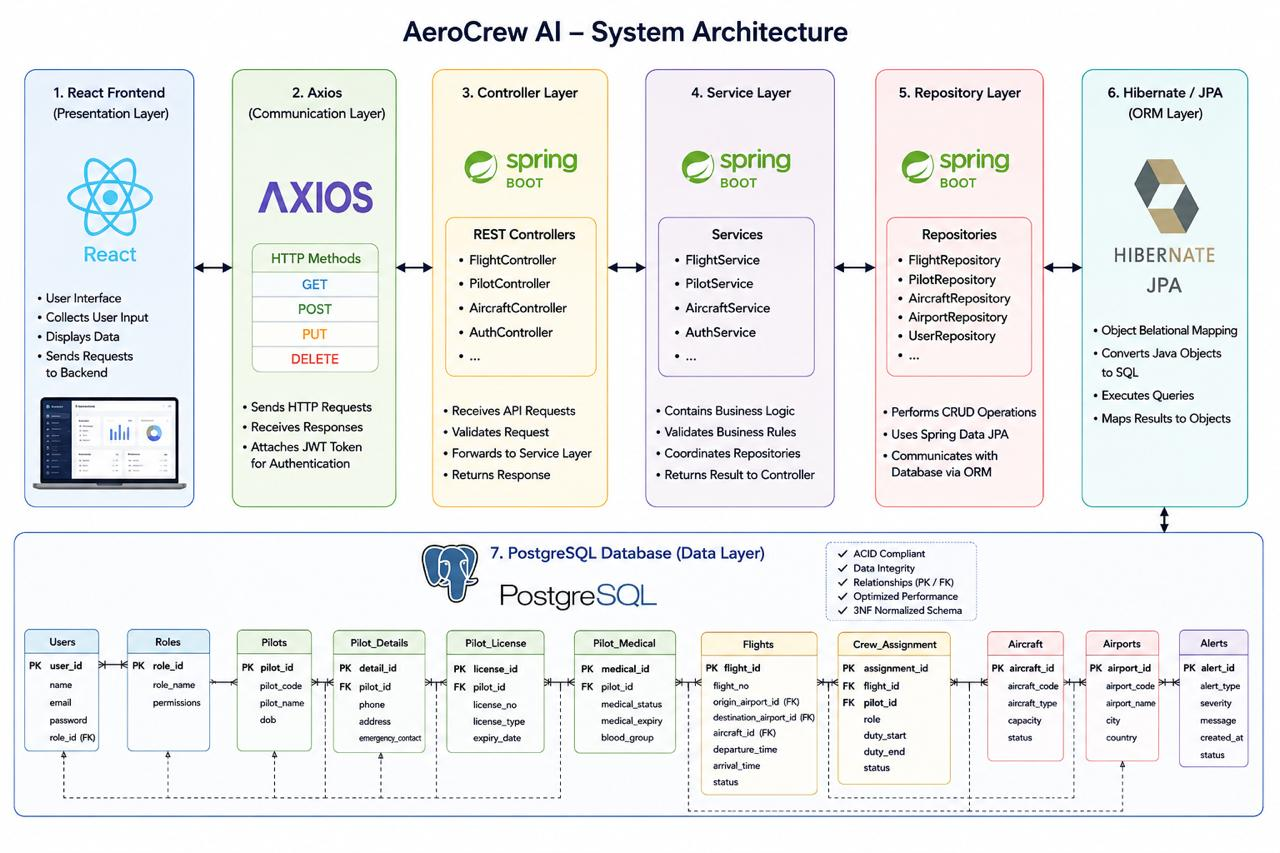
\includegraphics[width=1\textwidth]{blockdiagram.jpeg}
\caption{Overall Block Diagram of AeroCrew AI}
\label{fig:blockdiagram}
\end{figure}

The architecture separates presentation, business logic, and data persistence, ensuring modularity, maintainability, and scalability. External services are isolated through API integration, enabling future enhancements without affecting the core business logic.

%%%%%%%%%%%%%%%%%%%%%%%%%%%%%%%%%%%%%
% CHAPTER 3
%%%%%%%%%%%%%%%%%%%%%%%%%%%%%%%%%%%%%

\chapter{SYSTEM DESIGN}

This chapter presents the overall software design of AeroCrew AI. It explains the architecture, software modules, database organization, data flow, interface design, and reporting components that collectively support intelligent airline crew management and disruption recovery.

\section{SYSTEM ARCHITECTURE}

AeroCrew AI follows a modern three-tier enterprise architecture consisting of the Presentation Layer, Business Logic Layer, and Data Layer. This architecture promotes modularity, maintainability, scalability, and secure communication between software components.

The Presentation Layer consists of two independent client applications which are React Web Dashboard for Operations Control Center personnel and Native Android Application for airline pilots.


Both applications communicate with the backend through secured REST APIs.

The Business Layer is implemented using Spring Boot 3.5 and contains all business rules related to authentication, flight management, pilot management, disruption recovery, compliance validation, recommendation generation, notification management, and audit logging.

The Data Layer consists of PostgreSQL, which stores pilot records, aircraft information, flight schedules, recovery cases, notifications, weather information, audit logs, and operational statistics.

External services such as Firebase Cloud Messaging, weather APIs, and traffic services provide additional operational information that improves recommendation accuracy. Figure 3.1 presents the overall system architecture.

\begin{figure}[H]

\centering
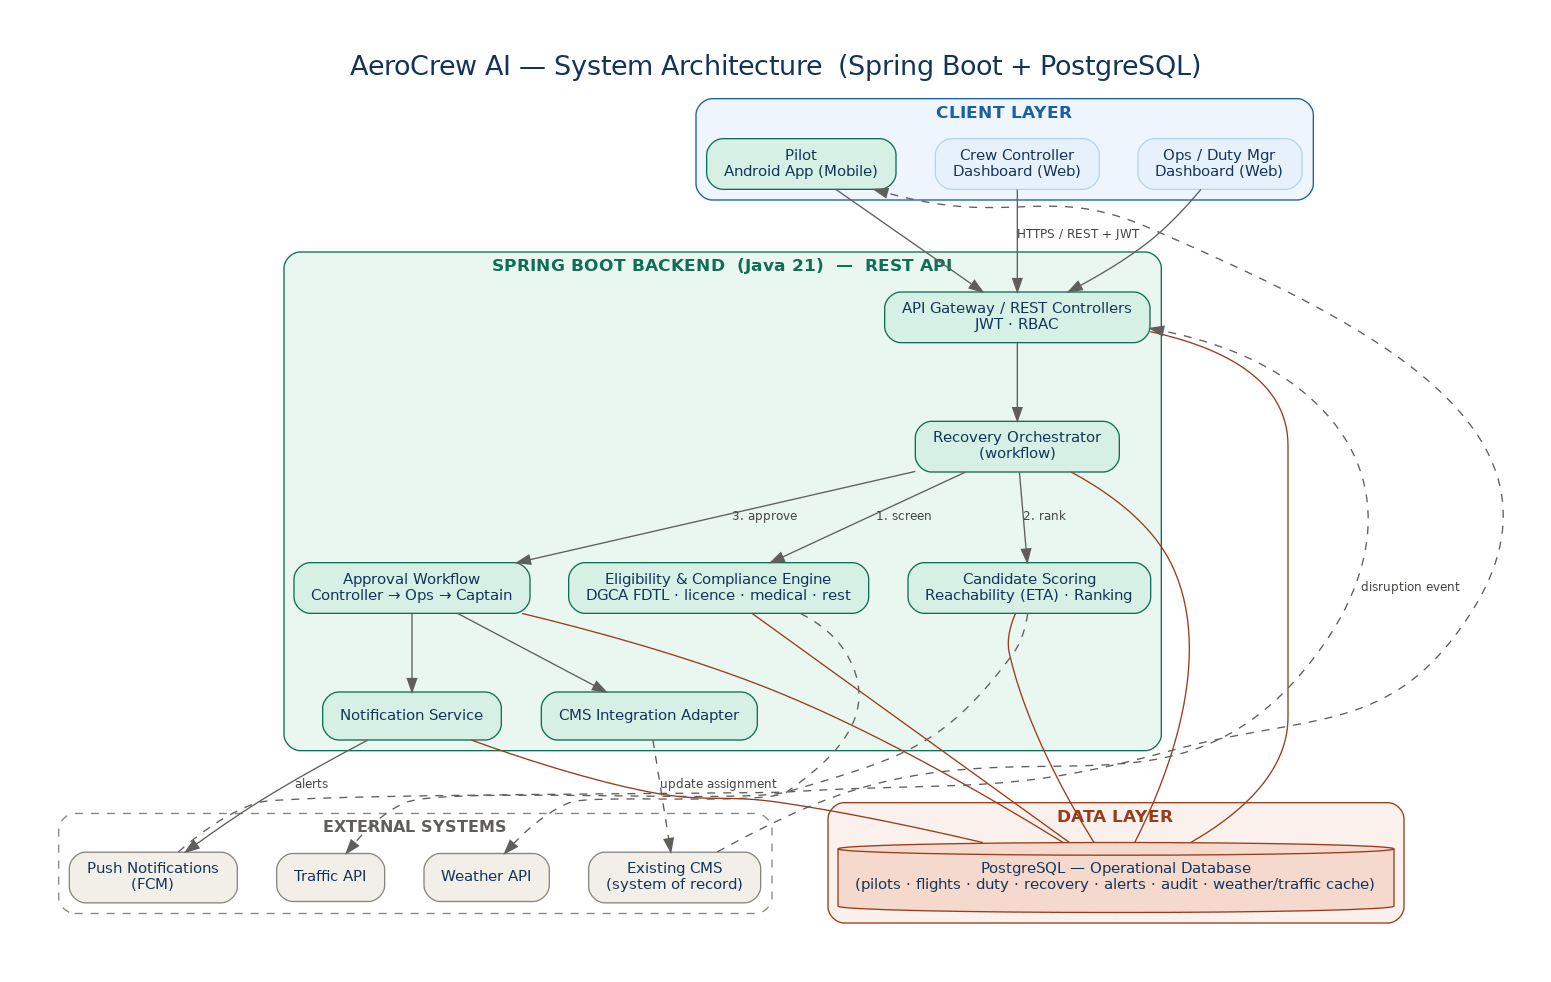
\includegraphics[width=1\textwidth]{systemoverallarch.png}

\caption{Overall System Architecture}

\label{fig:architecture}

\end{figure}

\section{MODULE DESIGN}

The AeroCrew AI platform has been divided into several independent functional modules following the divide-and-conquer principle of software engineering. Each module performs a specific responsibility while collaborating with other modules through clearly defined interfaces.

\subsection{Authentication Module}

Responsible for user login, registration, password encryption, JWT token generation, session validation, and role-based authorization.

\textbf{Major Functions}

\begin{itemize}

\item User Login

\item User Registration

\item JWT Authentication

\item Password Encryption

\item Role Management

\item Token Refresh

\end{itemize}

\subsection{Pilot Management Module}

This module manages pilot information including licenses, training history, medical certificates, standby status, duty history, and geographical location.

\textbf{Major Functions}

\begin{itemize}

\item Pilot Profile Management

\item Medical Record Verification

\item License Validation

\item Duty History

\item Standby Assignment

\item Availability Tracking

\end{itemize}

\subsection{Flight Management Module}

Responsible for maintaining airline schedules, aircraft assignments, operational status, airport information, and crew allocation.

\begin{itemize}

\item Flight Scheduling

\item Aircraft Allocation

\item Crew Assignment

\item Flight Monitoring

\item Airport Information

\end{itemize}

\subsection{Recovery Module}

The Recovery Module forms the core of AeroCrew AI. It automatically creates recovery cases, evaluates standby pilots, performs compliance validation, ranks candidates, and assists Operations Controllers during disruption recovery.

\begin{itemize}

\item Recovery Case Creation

\item Candidate Evaluation

\item Compliance Verification

\item Pilot Recommendation

\item Assignment Approval

\item Recovery Completion

\end{itemize}

\subsection{Dashboard Module}

Provides centralized operational monitoring through real-time visual dashboards displaying flights, delays, pilot availability, disruptions, and system statistics.

\subsection{Notification Module}

Responsible for sending push notifications to pilots using Firebase Cloud Messaging and notifying controllers about operational events.

\subsection{Audit Module}

Records every significant operational activity performed within the system, thereby ensuring accountability, transparency, and regulatory compliance.

\section{DATA FLOW DIAGRAM}

The Data Flow Diagram (DFD) represents the movement of information between system users, processing modules, external services, and the database, as shown in Figure 3.2.

\begin{figure}[H]

\centering

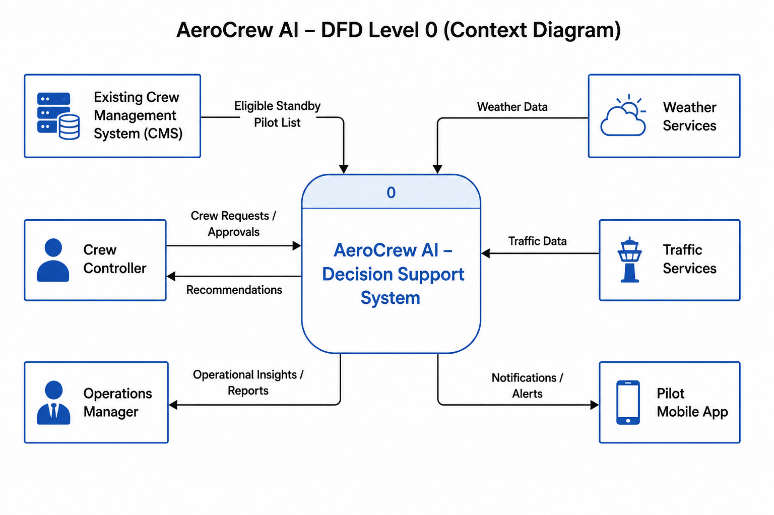
\includegraphics[width=1\textwidth]{dfd0.png}

\caption{Level-0 Data Flow Diagram}

\label{fig:dfd}

\end{figure}

The DFD illustrates how operational requests from airline controllers and pilots pass through the application server before interacting with the database and external services to produce meaningful responses.

\section{ENTITY RELATIONSHIP DIAGRAM}

The Entity Relationship (ER) Diagram models the logical relationships between the principal database entities used within AeroCrew AI, as shown in Figure 3.3.

\begin{figure}[H]

\centering

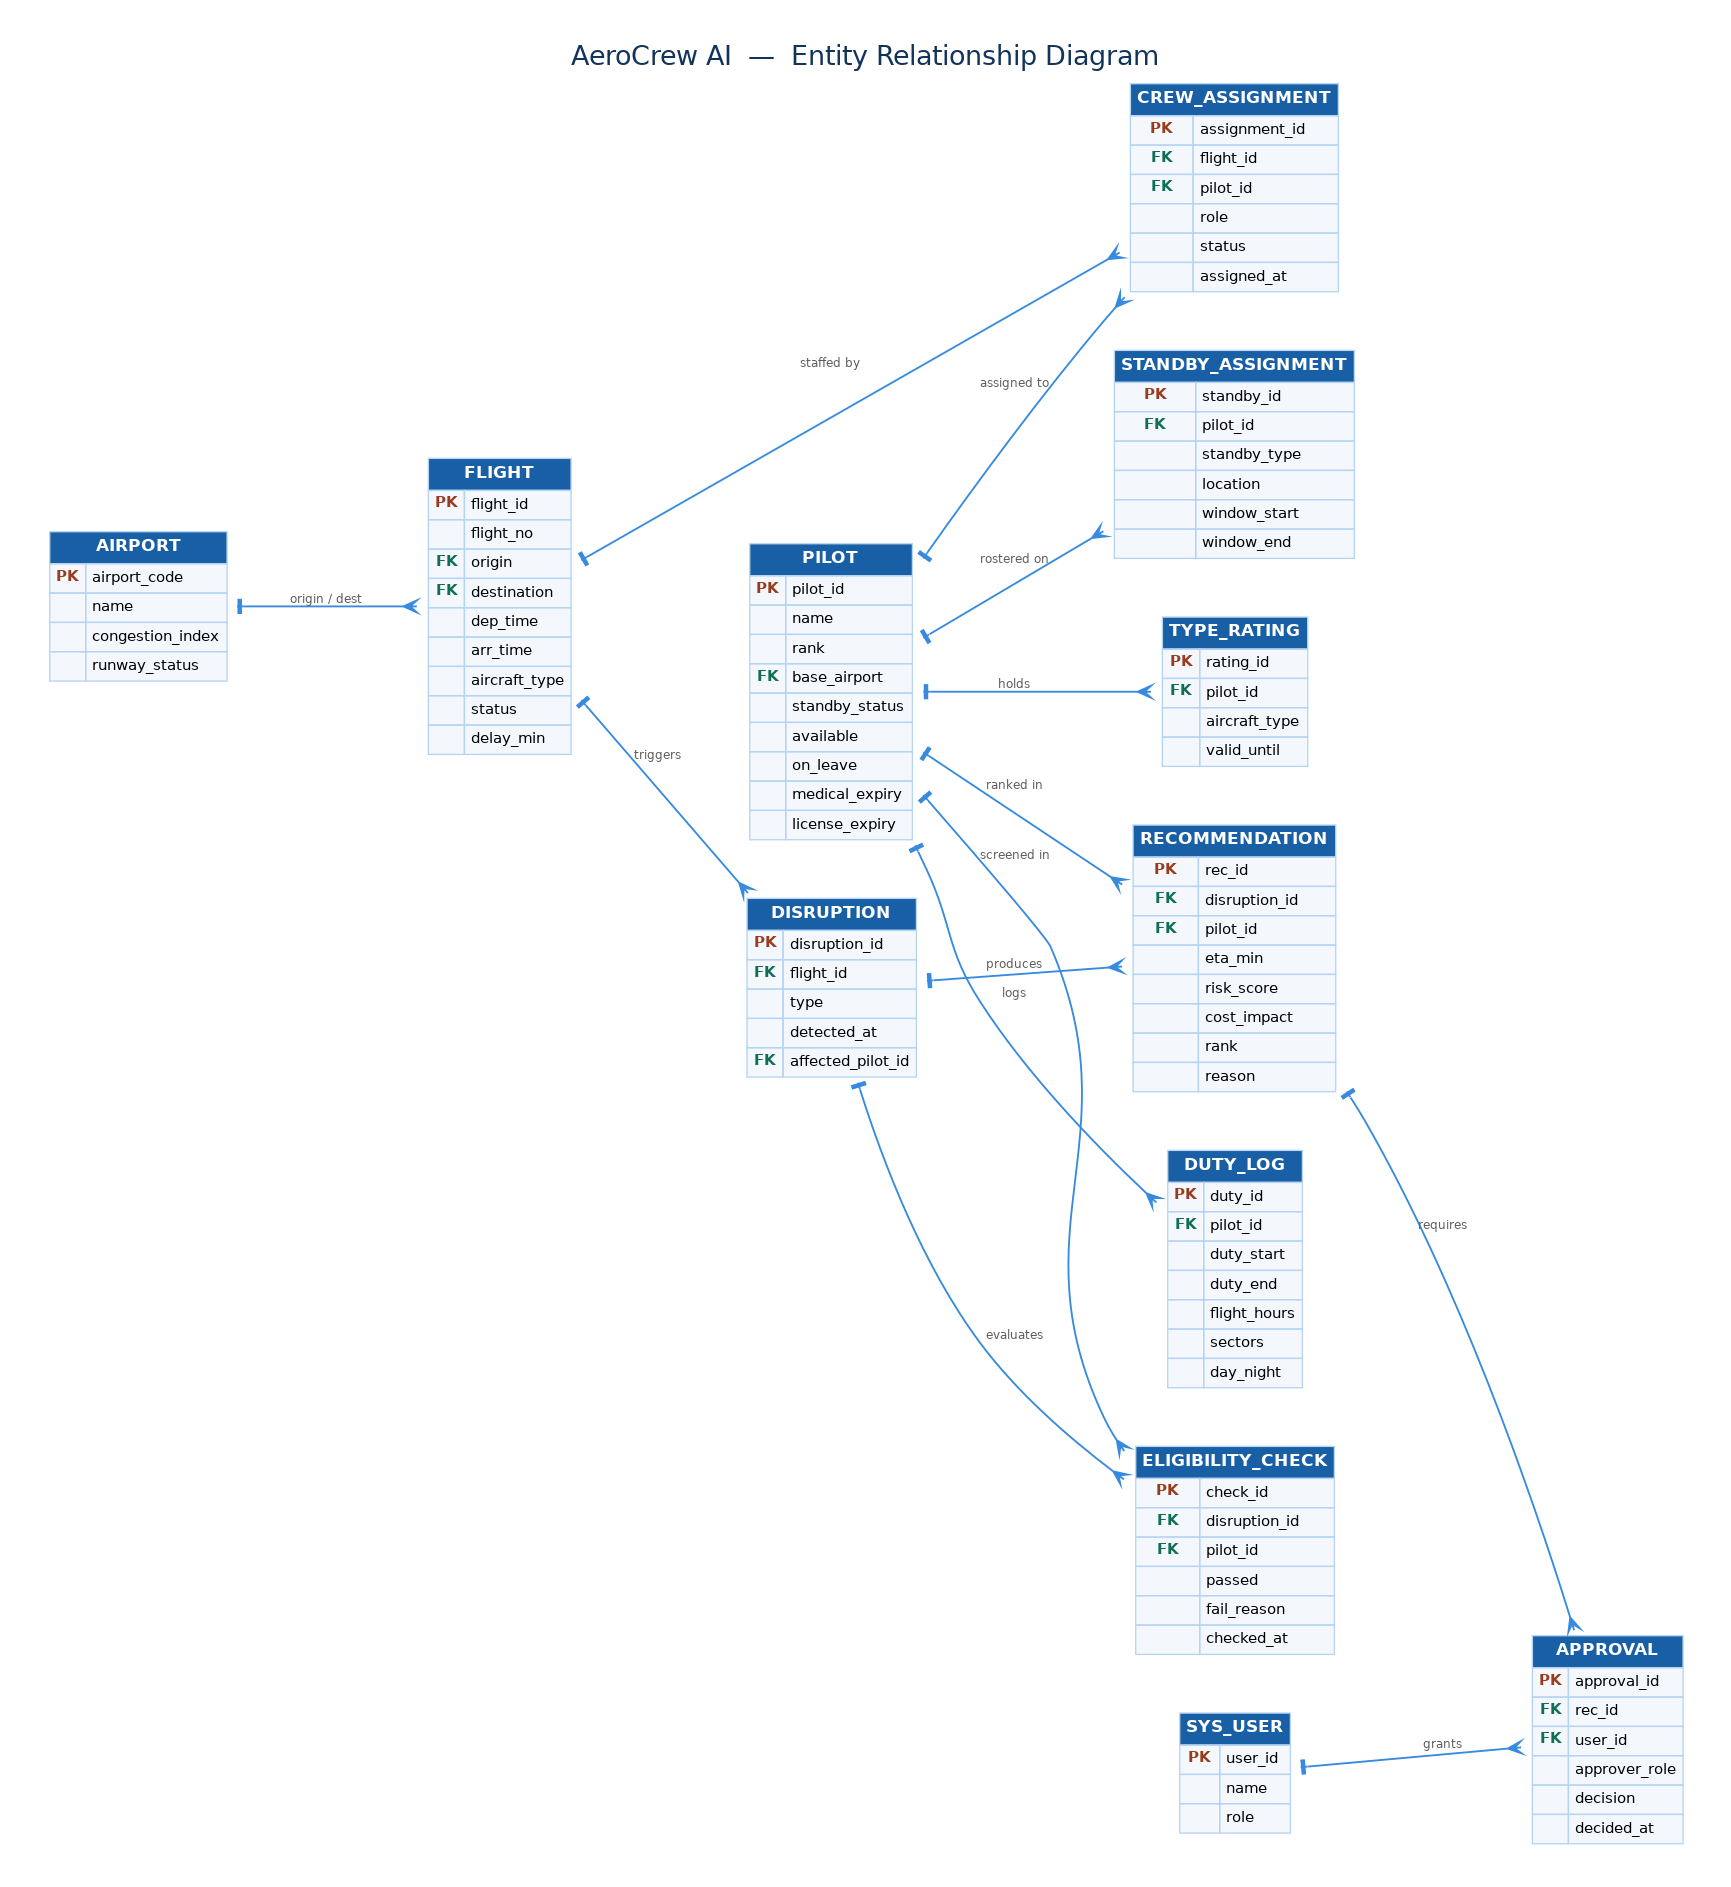
\includegraphics[width=1\textwidth]{erdiagram.png}

\caption{Entity Relationship Diagram}

\label{fig:erd}

\end{figure}

The primary entities include Users, Roles, Pilots, Flights, Aircraft, Recovery Cases, Recovery Candidates, Notifications, Weather Cache, Traffic Cache, and Audit Logs. These entities are interconnected through foreign-key relationships that ensure referential integrity and efficient querying.

\section{DATABASE DESIGN}

The AeroCrew AI system employs PostgreSQL as its primary relational database management system. The database has been designed using normalization principles to minimize redundancy while ensuring consistency, scalability, and high-performance data retrieval. Each major operational entity such as pilots, flights, aircraft, users, recovery cases, and operational logs is represented as an independent table connected through well-defined relationships.

The database architecture supports transactional processing, ensuring that critical operations such as crew assignments, recovery workflows, and notification generation are completed atomically. Foreign key constraints maintain referential integrity between related entities, while indexing is applied on frequently queried attributes such as pilot IDs, flight numbers, and recovery case identifiers to improve search performance.

The database design has been structured to support future enhancements, including predictive analytics, machine learning models, integration with airline reservation systems, and additional airport operations without requiring major structural changes.

\subsection{Table Design}

The following tables represent the major entities used in AeroCrew AI.

\subsubsection{Users Table}

Table 3.1 describes the structure of the Users table.

\begin{table}[H]
\centering
\caption{Users Table}

\begin{tabular}{|p{3.5cm}|p{2.5cm}|p{5cm}|p{2.5cm}|}

\hline
\textbf{Column} & \textbf{Datatype} & \textbf{Description} & \textbf{Constraint}\\
\hline

user\_id & BIGINT & Unique User Identifier & Primary Key\\
\hline

name & VARCHAR(100) & User Name & Not Null\\
\hline

email & VARCHAR(100) & Login Email & Unique\\
\hline

password & VARCHAR(255) & Encrypted Password & Not Null\\
\hline

role\_id & BIGINT & Assigned User Role & Foreign Key\\
\hline

status & VARCHAR(20) & Account Status & Default ACTIVE\\
\hline

\end{tabular}

\end{table}

\subsubsection{Pilot Table}

Table 3.2 describes the structure of the Pilot table.

\begin{table}[H]

\centering

\caption{Pilot Table}

\begin{tabular}{|p{3.5cm}|p{2.5cm}|p{5cm}|p{2.5cm}|}

\hline

pilot\_id & BIGINT & Pilot Identifier & Primary Key\\
\hline

pilot\_name & VARCHAR(100) & Pilot Name & Not Null\\
\hline

license\_number & VARCHAR(50) & License Number & Unique\\
\hline

medical\_status & VARCHAR(20) & Medical Fitness & Not Null\\
\hline

standby\_status & VARCHAR(20) & Current Availability & Not Null\\
\hline

current\_location & VARCHAR(100) & Current Location & --\\
\hline

\end{tabular}

\end{table}

\subsubsection{Flight Table}

Table 3.3 describes the structure of the Flight table.

\begin{table}[H]

\centering

\caption{Flight Table}

\begin{tabular}{|p{3.5cm}|p{2.5cm}|p{5cm}|p{2.5cm}|}

\hline

flight\_id & BIGINT & Flight Identifier & Primary Key\\
\hline

flight\_number & VARCHAR(30) & Flight Number & Unique\\
\hline

departure & VARCHAR(50) & Departure Airport & Not Null\\
\hline

arrival & VARCHAR(50) & Arrival Airport & Not Null\\
\hline

departure\_time & TIMESTAMP & Scheduled Departure & Not Null\\
\hline

status & VARCHAR(30) & Flight Status & Not Null\\
\hline

\end{tabular}

\end{table}

\subsubsection{Recovery Case Table}

Table 3.4 describes the structure of the Recovery Case table.

\begin{table}[H]

\centering

\caption{Recovery Case Table}

\begin{tabular}{|p{3.5cm}|p{2.5cm}|p{5cm}|p{2.5cm}|}

\hline

case\_id & BIGINT & Recovery Case Identifier & Primary Key\\
\hline

flight\_id & BIGINT & Flight Reference & Foreign Key\\
\hline

disruption\_type & VARCHAR(100) & Type of Disruption & Not Null\\
\hline

status & VARCHAR(30) & Recovery Status & OPEN\\
\hline

created\_time & TIMESTAMP & Creation Time & Not Null\\
\hline

resolved\_time & TIMESTAMP & Resolution Time & Nullable\\
\hline

\end{tabular}

\end{table}

\subsection{Data Integrity and Constraints}

The integrity of operational data is critical for ensuring airline safety and regulatory compliance. AeroCrew AI employs multiple validation and security mechanisms to maintain data consistency, reliability, and integrity throughout the system. Primary keys are used to uniquely identify each database record, while foreign key constraints maintain relationships between related entities. Unique constraints prevent duplicate flight numbers, user accounts, and pilot licenses, and NOT NULL constraints ensure that mandatory operational information is always available.

Transaction management ensures that critical operations, such as crew assignments, are executed atomically. Passwords are securely stored using BCrypt encryption, while role-based authorization prevents unauthorized users from accessing restricted functionality. Input validation is performed on both the client side and server side to ensure that invalid or inappropriate data is not processed by the system.

The system also implements audit logging to record significant modifications and operational activities, thereby improving accountability and traceability. Furthermore, recovery workflows are designed to automatically roll back changes if any step fails, helping maintain database consistency and preventing incomplete or inconsistent operational transactions.

\subsection{Data Dictionary}

Table 3.5 presents a sample of the data dictionary maintained for AeroCrew AI.

\begin{table}[H]

\centering

\caption{Sample Data Dictionary}

\begin{tabular}{|p{3cm}|p{3cm}|p{1.5cm}|p{1.5cm}|p{5cm}|}

\hline

\textbf{Field} &
\textbf{Datatype} &
\textbf{Min} &
\textbf{Max} &
\textbf{Description}\\

\hline

user\_id &
BIGINT &
1 &
999999 &
Unique User Identifier\\

\hline

pilot\_name &
VARCHAR &
1 &
100 &
Pilot Full Name\\

\hline

license\_number &
VARCHAR &
5 &
50 &
Pilot License Number\\

\hline

flight\_number &
VARCHAR &
3 &
20 &
Flight Code\\

\hline

status &
VARCHAR &
3 &
20 &
Current Operational Status\\

\hline

\end{tabular}

\end{table}

\section{INTERFACE AND PROCEDURAL DESIGN}

AeroCrew AI has been designed following modern Human-Computer Interaction (HCI) principles. The interface emphasizes simplicity, consistency, responsiveness, and operational efficiency. Since airline controllers operate in high-pressure environments, the dashboard presents only the most relevant operational information while minimizing unnecessary navigation.

The application adopts a responsive design, enabling seamless access from desktop systems used in the Operations Control Center and Android devices used by pilots. Standardized color coding is employed throughout the interface to represent flight status, crew availability, disruption severity, and operational alerts. Interactive tables, charts, and notification panels enable controllers to monitor multiple operational events simultaneously.

\subsection{User Interface Design}

The user interface consists of several functional screens.

\begin{enumerate}

\item Login Page

\item Dashboard

\item Pilot Management

\item Flight Management

\item Recovery Dashboard

\item Recovery Candidate Ranking Screen

\item Notification Center

\item User Management

\item Reports Dashboard

\item Mobile Pilot Application

\end{enumerate}

Each screen follows a consistent layout consisting of:

\begin{itemize}

\item Navigation Sidebar

\item Header

\item Search Panel

\item Data Tables

\item Action Buttons

\item Status Cards

\item Charts and Analytics

\end{itemize}

Figure 3.4 presents a sample layout of the operations dashboard.

\begin{figure}[H]

\centering

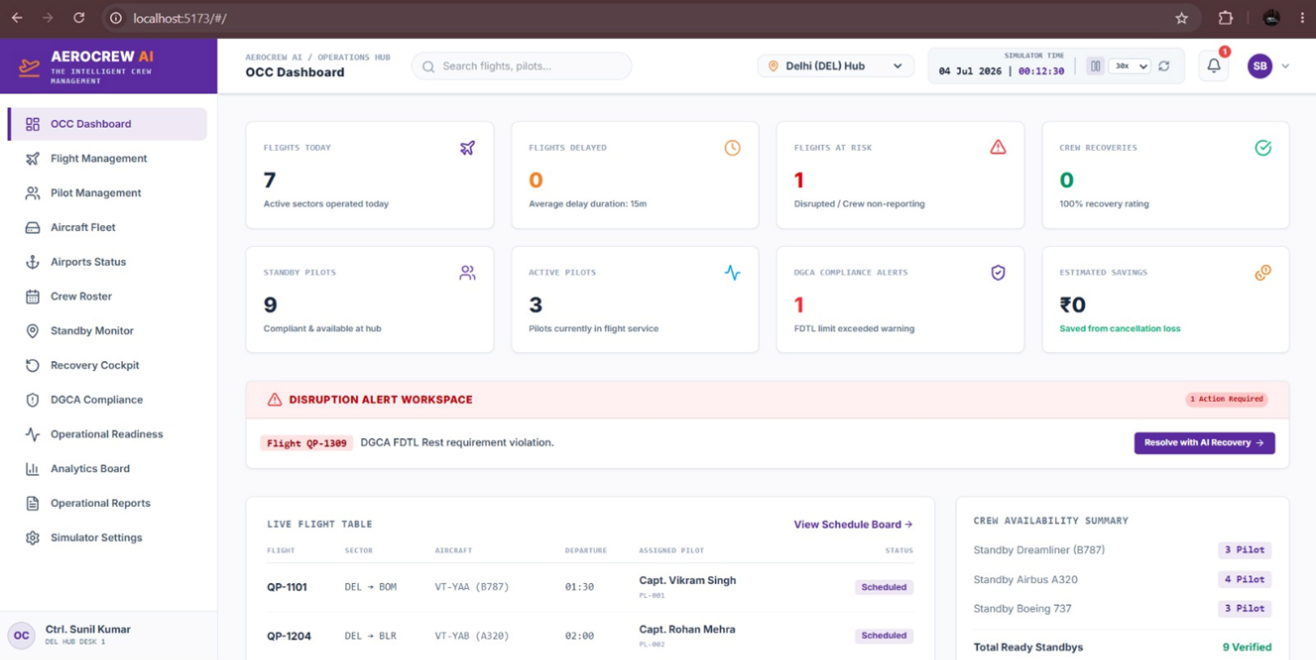
\includegraphics[width=1\textwidth]{dashboard.png}

\caption{Sample Dashboard Layout}

\end{figure}

\section{REPORTS DESIGN}

The reporting module enables airline management to analyze operational performance and make strategic decisions based on historical and real-time information. Reports are generated dynamically and can be exported for administrative, regulatory, and operational purposes.

Major reports generated by the system include:

\begin{itemize}

\item Flight Operations Summary Report

\item Crew Availability Report

\item Standby Pilot Report

\item Recovery Case Report

\item Flight Delay Analysis Report

\item Crew Utilization Report

\item Compliance Validation Report

\item Notification Activity Report

\item Audit Log Report

\item Dashboard Performance Statistics

\end{itemize}

Each report allows filtering based on date range, flight number, airport, pilot, recovery status, operational controller, or disruption type. Reports may be exported in PDF, Excel, or CSV formats for further analysis and archival.

\section*{CHAPTER SUMMARY}
\addcontentsline{toc}{section}{Chapter Summary}

This chapter presented the complete design of the AeroCrew AI system, including its architecture, functional modules, database schema, interface design, and reporting framework. The proposed three-tier architecture, modular organization, normalized relational database, and secure REST-based communication provide a scalable, maintainable, and enterprise-ready solution for intelligent airline crew management. The design establishes a strong foundation for future implementation, testing, deployment, and integration with advanced Artificial Intelligence and predictive analytics capabilities.

%%%%%%%%%%%%%%%%%%%%%%%%%%%%%%%%%%%%%
% CHAPTER 4
%%%%%%%%%%%%%%%%%%%%%%%%%%%%%%%%%%%%%

\chapter{IMPLEMENTATION}

This chapter describes how the design of AeroCrew AI presented in Chapter 3 was translated into a working software system. It covers the implementation approach adopted, the coding standards followed, representative code snippets from key modules, and screenshots demonstrating the functionality of the developed system.

\section{IMPLEMENTATION APPROACHES}

The implementation of AeroCrew AI followed an Incremental and Agile development methodology, in which the system was developed and delivered through small, functional increments rather than as a single monolithic release. Each increment focused on a specific module, including authentication, pilot management, flight management, disruption recovery, and the mobile notification system. This approach allowed the team to test and validate functionality at an early stage and continuously refine the system based on feedback.

The implementation process began with requirement breakdown, where the functional requirements identified in Chapter 2 were divided into smaller, implementable user stories and tasks. This was followed by sprint-based development, in which development was organized into short iterations, with each sprint delivering a testable increment of the system in accordance with Agile project management practices.

The backend-first development approach was then adopted, with core services such as authentication, pilot management, flight management, and the recovery engine implemented using Spring Boot. REST APIs were subsequently developed to expose these backend functionalities. In parallel, the React web dashboard was developed and integrated with the backend once the required API endpoints became stable.

The mobile application was developed using Android Studio and integrated with the backend through the same REST API layer. Firebase Cloud Messaging was also incorporated to support push notifications for pilots. Throughout the development process, continuous testing was performed, with each increment undergoing unit and integration testing before being merged into the main codebase. This helped minimize the propagation of defects to subsequent development stages.

Finally, Git and GitHub were used for version control throughout the project to manage source code, track changes, and support collaboration among team members. Overall, the incremental approach enabled the team to manage system complexity, accommodate design refinements as development progressed, and maintain a working version of the system at the end of each development cycle.


\section{CODING STANDARD}

To ensure readability, maintainability, and consistency across the codebase, several coding standards were adopted throughout the development of AeroCrew AI. These standards establish a consistent approach to naming, project organization, API development, error handling, documentation, frontend development, and version control.

Naming conventions were followed throughout the application. Java classes use PascalCase, such as PilotService, while methods and variables follow camelCase, such as getEligiblePilots(). Constants are written using UPPER_SNAKE_CASE to clearly distinguish them from other variables and methods.

The backend follows a structured package organization to maintain separation of concerns. The code is divided into layered packages such as controller, service, repository, entity, dto, and config. This organization improves maintainability and makes it easier to modify or extend individual components without affecting unrelated parts of the application.

For RESTful API design, endpoints follow standard REST conventions by using plural resource names such as /api/pilots and /api/flights. Appropriate HTTP methods, including GET, POST, PUT, and DELETE, are used according to the operation being performed. Exception handling is centralized using Spring's @ControllerAdvice, ensuring that errors are handled consistently and meaningful responses are returned to clients.

Code documentation is also maintained throughout the project. Non-trivial methods include brief comments describing their purpose, parameters, and return values, while complex business logic, such as the compliance validation and candidate ranking engines, is documented using inline comments to improve understanding and maintainability.

For the frontend, React components follow functional component and Hooks conventions. Component names use PascalCase, and files are organized according to their respective features. This provides a consistent structure and makes the frontend codebase easier to navigate and maintain.

Finally, version control practices were followed using Git and GitHub. Commits use consistent prefixes such as feat:, fix:, and refactor: to clearly indicate the type of change being made. Feature branches are used for individual development tasks and are merged into the main branch after review, supporting organized and collaborative software development.

\section{CODING DETAILS}

This section presents representative code excerpts from key modules of AeroCrew AI. Only the essential portions of the implementation are shown, with inline comments explaining the purpose of each segment.

\subsection{Pilot Compliance Validation}

The following snippet illustrates the core logic used to validate a standby pilot's eligibility against DGCA Flight Duty Time Limitation regulations before the candidate is considered for recovery recommendations.

\begin{singlespace}
\begin{verbatim}
// Validates whether a pilot is eligible for assignment
// based on DGCA FDTL regulations
public boolean isPilotEligible(Pilot pilot, Flight flight) {

    // Check license validity
    if (!pilot.getLicenseStatus().equals("VALID")) {
        return false;
    }

    // Check medical fitness
    if (!pilot.getMedicalStatus().equals("FIT")) {
        return false;
    }

    // Check mandatory rest period compliance
    Duration restPeriod = Duration.between(
        pilot.getLastDutyEndTime(), flight.getDepartureTime());

    if (restPeriod.toHours() < MINIMUM_REST_HOURS) {
        return false;
    }

    // Check aircraft type rating
    if (!pilot.getAircraftRatings().contains(flight.getAircraftType())) {
        return false;
    }

    return true;
}
\end{verbatim}
\end{singlespace}

\subsection{Candidate Ranking Engine}

The candidate ranking engine scores each eligible standby pilot using a weighted combination of travel time, availability, and operational suitability.

\begin{singlespace}
\begin{verbatim}
// Computes a ranking score for an eligible candidate
public double computeRankingScore(Pilot pilot, double travelTimeMinutes) {

    double travelScore = Math.max(0, 100 - travelTimeMinutes);
    double availabilityScore = pilot.isStandbyReady() ? 100 : 50;
    double experienceScore = Math.min(pilot.getFlightHours() / 10.0, 100);

    // Weighted sum: travel time is prioritized, followed by
    // availability and experience
    return (0.5 * travelScore)
         + (0.3 * availabilityScore)
         + (0.2 * experienceScore);
}
\end{verbatim}
\end{singlespace}

\subsection{Recovery Case REST Endpoint}

The following controller method exposes an endpoint that returns ranked standby pilot recommendations for a given recovery case.

\begin{singlespace}
\begin{verbatim}
@GetMapping("/api/recovery-cases/{caseId}/recommendations")
public ResponseEntity<List<PilotRecommendationDto>> getRecommendations(
        @PathVariable Long caseId) {

    // Delegate to the recovery service to compute
    // eligible and ranked candidates
    List<PilotRecommendationDto> recommendations =
            recoveryService.getRankedCandidates(caseId);

    return ResponseEntity.ok(recommendations);
}
\end{verbatim}
\end{singlespace}

\section{SCREEN SHOTS}

This section presents representative screenshots of the AeroCrew AI web application and
the integrated Android pilot application. The screenshots demonstrate the major operational
modules, including flight management, pilot management, fleet monitoring, crew roster
management, standby monitoring, recovery operations, DGCA compliance, operational
readiness, analytics, reporting, and the pilot-facing mobile application.

\subsection{Web Application Screenshots}

The AeroCrew AI web application provides the Operations Control Center with a centralized
interface for monitoring flights, crew, aircraft, airport conditions, compliance status, and
recovery activities. The following screenshots demonstrate the major modules implemented
for airline operations management.

\subsubsection{OCC Dashboard}

The OCC Dashboard provides an overview of the current operational situation. It displays
key indicators such as flights operated, delayed flights, flights at risk, crew recoveries,
standby pilots, active pilots, DGCA compliance alerts, estimated savings, and active
disruption alerts.

\begin{figure}[H]
\centering
\includegraphics[width=0.98\textwidth]{occ dashboard.png}
\caption{AeroCrew AI OCC Dashboard}
\label{fig:occ_dashboard}
\end{figure}

\subsubsection{Flight Management}

The Flight Management module provides a centralized list of scheduled and disrupted
flights along with assigned pilots, aircraft types, departure times, routes, and operational
status. The flight details panel also provides crew compliance information and disruption
simulation controls.

\begin{figure}[H]
\centering
\includegraphics[width=0.98\textwidth]{flight management.png}
\caption{Flight Management Module}
\label{fig:flight_management}
\end{figure}

\subsubsection{Pilot Management}

The Pilot Management module maintains the pilot registry and displays pilot IDs, names,
aircraft ratings, medical expiry dates, license status, cumulative flight hours, and current
crew status.

\begin{figure}[H]
\centering
\includegraphics[width=0.98\textwidth]{pilot management.png}
\caption{Pilot Management Module}
\label{fig:pilot_management}
\end{figure}

\subsubsection{Aircraft Fleet}

The Aircraft Fleet module provides information about aircraft registration, aircraft type,
base location, scheduled maintenance checks, accumulated flight hours, and operational
status. The fleet detail panel provides additional airworthiness and assignment information.

\begin{figure}[H]
\centering
\includegraphics[width=0.98\textwidth]{aircraft fleet.png}
\caption{Aircraft Fleet Management Module}
\label{fig:aircraft_fleet}
\end{figure}

\subsubsection{Airport Status}

The Airport Status module presents airport-level operational information including weather
conditions, visibility, congestion, runway status, terminal conditions, and relevant
operational messages.

\begin{figure}[H]
\centering
\includegraphics[width=0.98\textwidth]{airport status.png}
\caption{Airport Status Module}
\label{fig:airport_status}
\end{figure}

\subsubsection{Crew Roster}

The Crew Roster module provides daily and weekly views of pilot assignments. It displays
pilot IDs, ratings, active or standby status, and the flights or sectors assigned to each
pilot.

\begin{figure}[H]
\centering
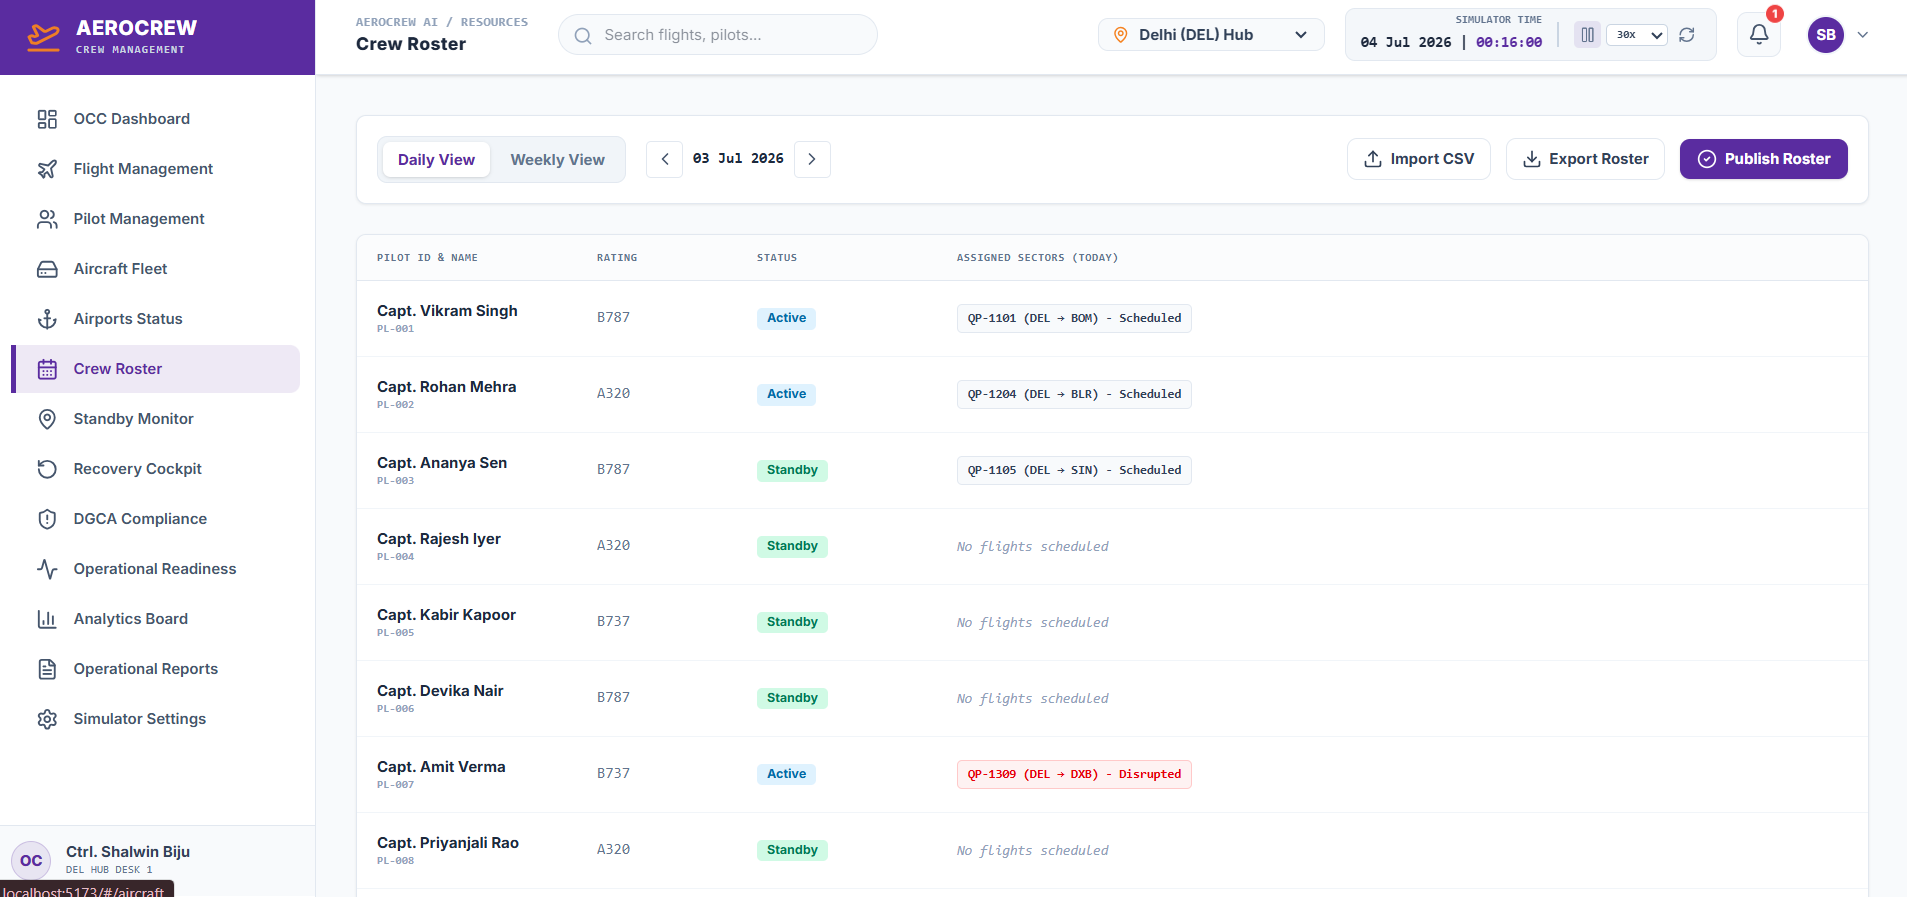
\includegraphics[width=0.98\textwidth]{Crew roaster.png}
\caption{Crew Roster Module}
\label{fig:crew_roster}
\end{figure}

\subsubsection{Standby Monitor}

The Standby Monitor provides a real-time view of available standby pilots and their
locations relative to the hub. It includes estimated arrival times, travel modes, traffic
conditions, readiness indicators, and a map showing the geographical distribution of
standby crew.

\begin{figure}[H]
\centering
\includegraphics[width=0.98\textwidth]{standby monitor.png}
\caption{Standby Monitor Module}
\label{fig:standby_monitor}
\end{figure}

\subsubsection{Recovery Cockpit}

The Recovery Cockpit supports disruption recovery by displaying disrupted flights, the
reason for disruption, the incident timeline, eligible standby pilots, DGCA checks, estimated
arrival times, FDTL rest information, and AI-generated recommendation scores. It also
provides a disruption cost estimator and savings information.

\begin{figure}[H]
\centering
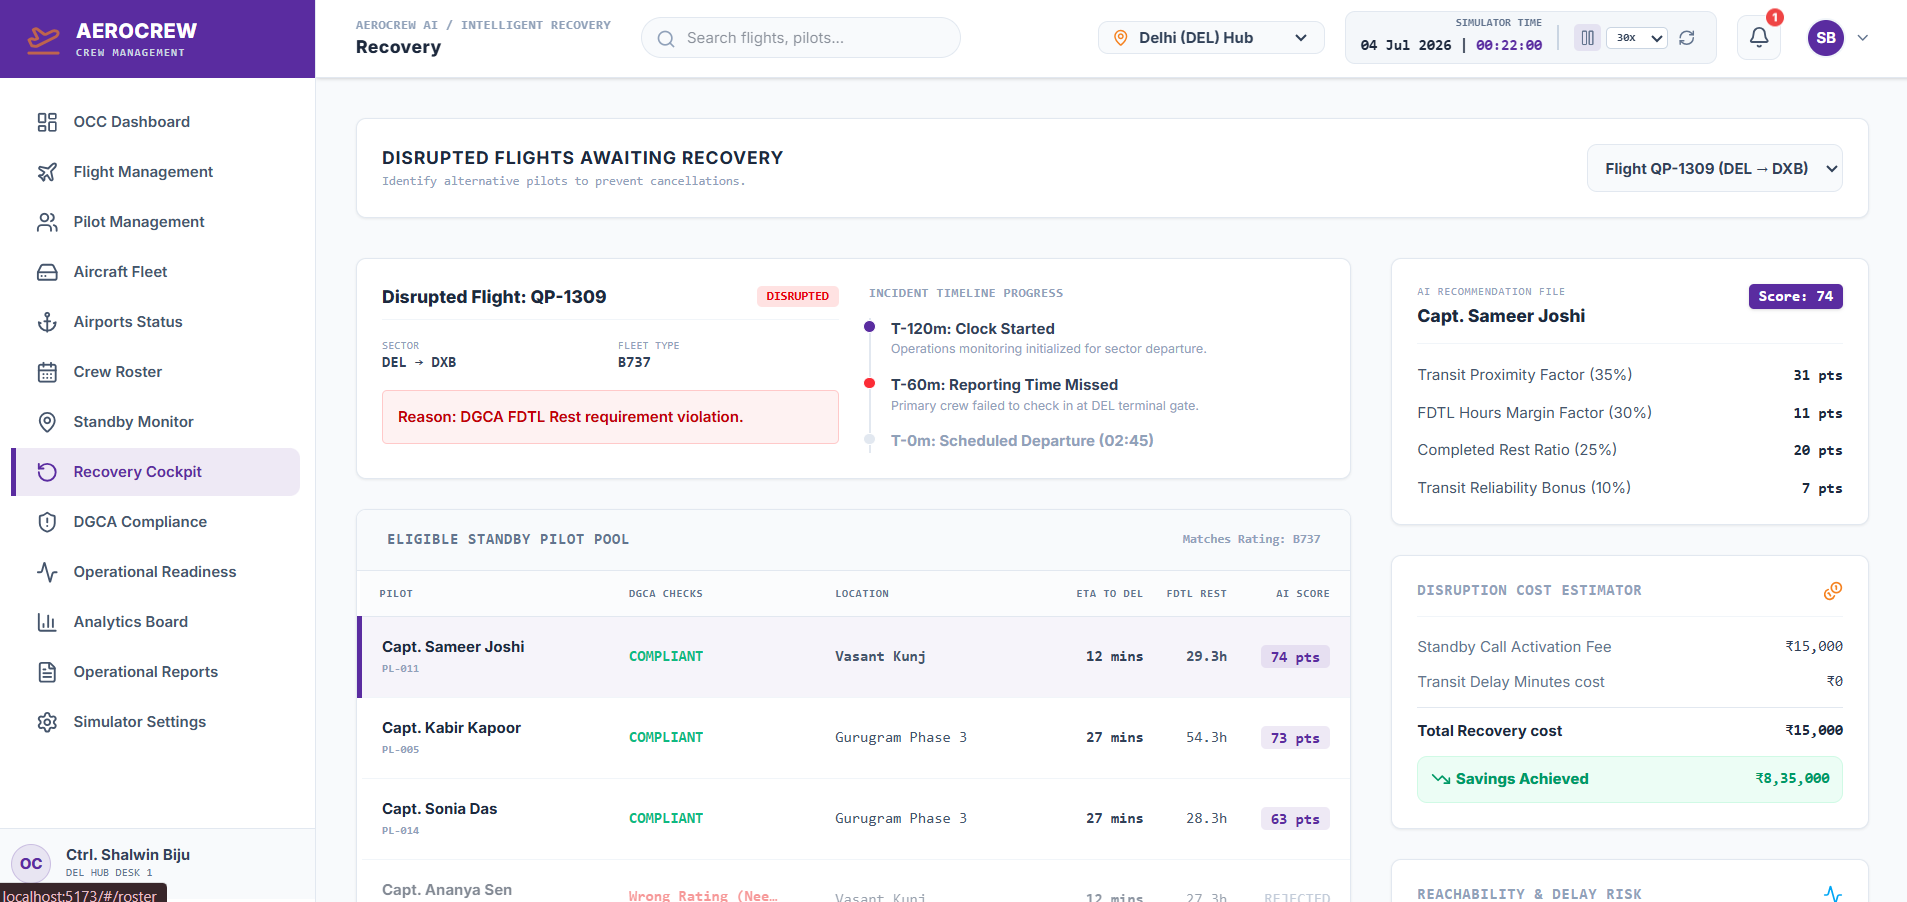
\includegraphics[width=0.98\textwidth]{Recovery cockpit.png}
\caption{AI Crew Recovery Cockpit}
\label{fig:recovery_cockpit}
\end{figure}

\subsubsection{DGCA Compliance}

The DGCA Compliance module provides a reference for applicable flight duty and rest
requirements and monitors pilot compliance. The interface displays license and medical
verification statistics, active rest infractions, flight-hour limits, and individual pilot
compliance status.

\begin{figure}[H]
\centering
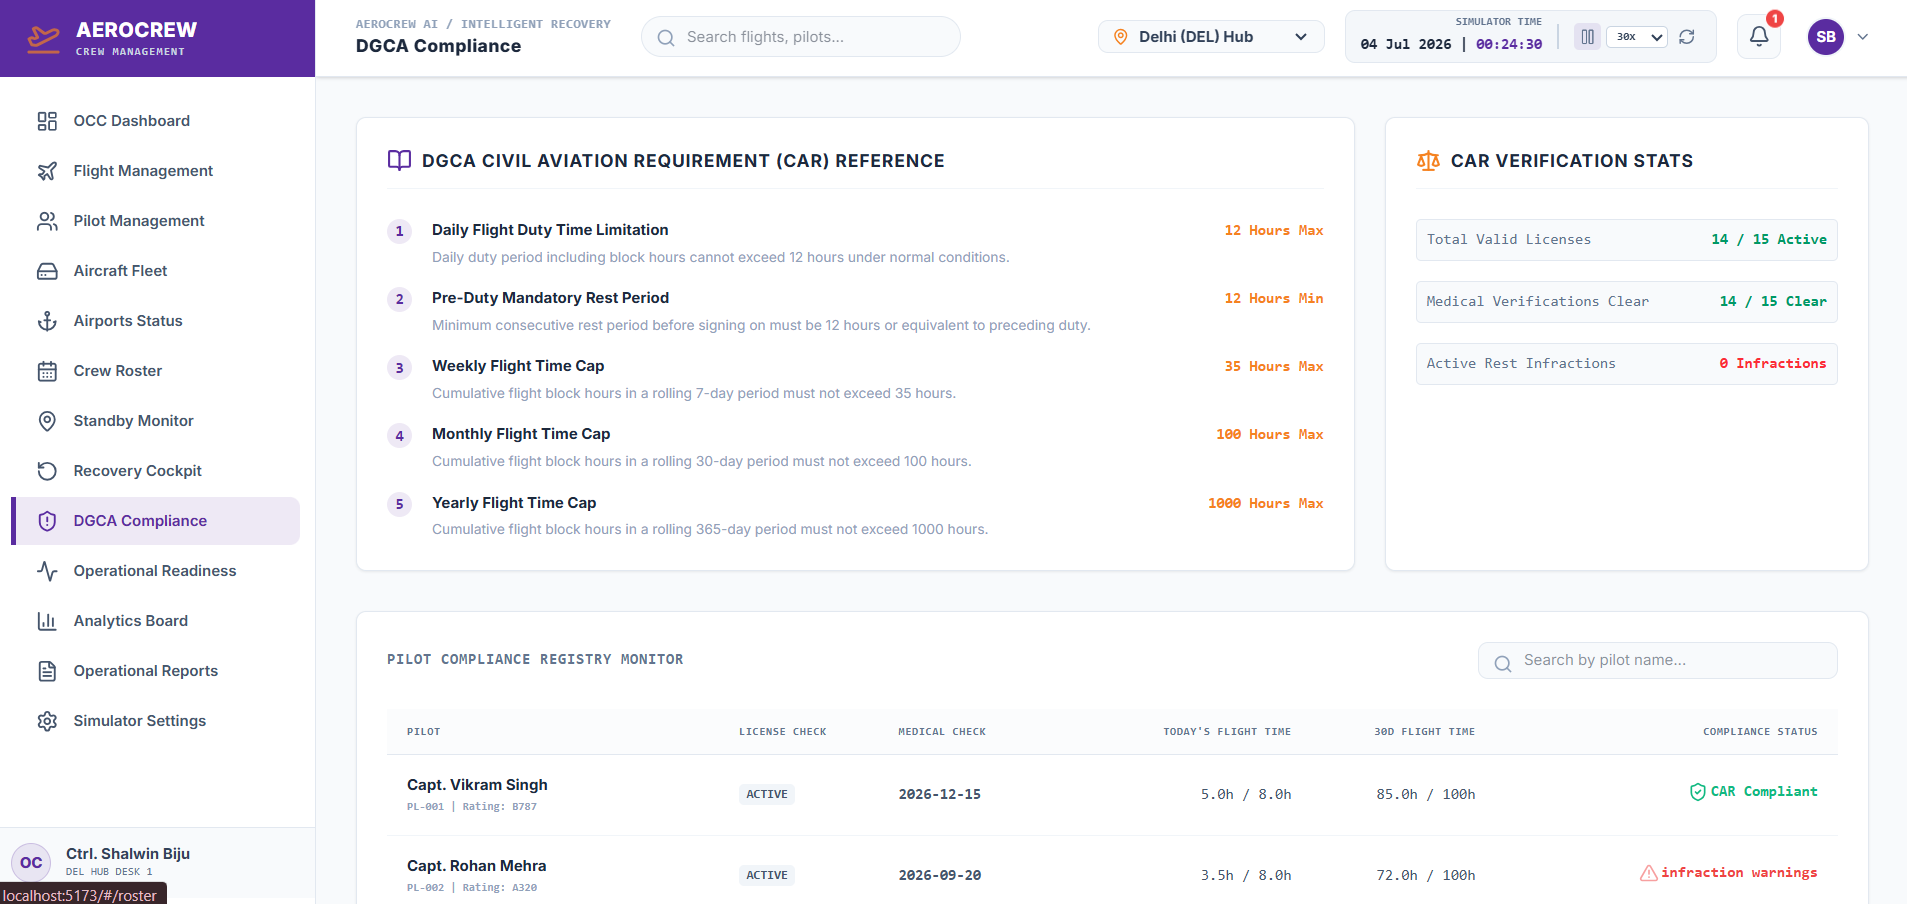
\includegraphics[width=0.98\textwidth]{DGCA compilance.png}
\caption{DGCA Compliance Module}
\label{fig:dgca_compliance}
\end{figure}

\subsubsection{Operational Readiness}

The Operational Readiness module evaluates the reachability of standby pilots by combining
travel distance, travel mode, weather multipliers, traffic multipliers, and adjusted estimated
arrival time. The resulting readiness rating supports rapid selection of operationally
suitable standby crew.

\begin{figure}[H]
\centering
\includegraphics[width=0.98\textwidth]{operational readiness.png}
\caption{Operational Readiness Module}
\label{fig:operational_readiness}
\end{figure}

\subsubsection{Analytics Board}

The Analytics Board provides operational performance indicators and visual analytics such
as recovery success rate, standby swaps, operational cost savings, average dispatch time,
crew fleet utilization, operational damage prevented by hub, and disruption-prevention
savings trends.

\begin{figure}[H]
\centering
\includegraphics[width=0.98\textwidth]{analytics board.png}
\caption{Analytics Board}
\label{fig:analytics_board}
\end{figure}

\subsubsection{Operational Reports}

The Operational Reports module allows controllers to select report types and reporting
periods and generate audit reports. The interface also supports downloading reports as PDF
and exporting report data in CSV format.

\begin{figure}[H]
\centering
\includegraphics[width=0.98\textwidth]{operational reports.png}
\caption{Operational Reports Module}
\label{fig:operational_reports}
\end{figure}

\subsection{Android Mobile Application}

The Android mobile application was developed as an integrated pilot-facing component of
AeroCrew AI. It extends the platform to mobile devices and provides pilots with access to
flight information, readiness status, operational alerts, crew recovery requests, and profile
information. The application is designed to support timely communication between airline
operations and pilots during normal operations and disruption recovery.

\subsubsection{Welcome and Authentication Screens}

The Android application begins with a dedicated welcome screen followed by pilot
authentication. The authentication interface allows the pilot to sign in using the registered
pilot credentials.

\begin{figure}[H]
\centering
\begin{minipage}[t]{0.43\textwidth}
    \centering
    
\includegraphics[width=\textwidth]{Welcome Screen.jpeg}
    \captionof{figure}{Android Welcome Screen}
    \label{fig:android_welcome}
\end{minipage}
\hfill
\begin{minipage}[t]{0.43\textwidth}
    \centering
    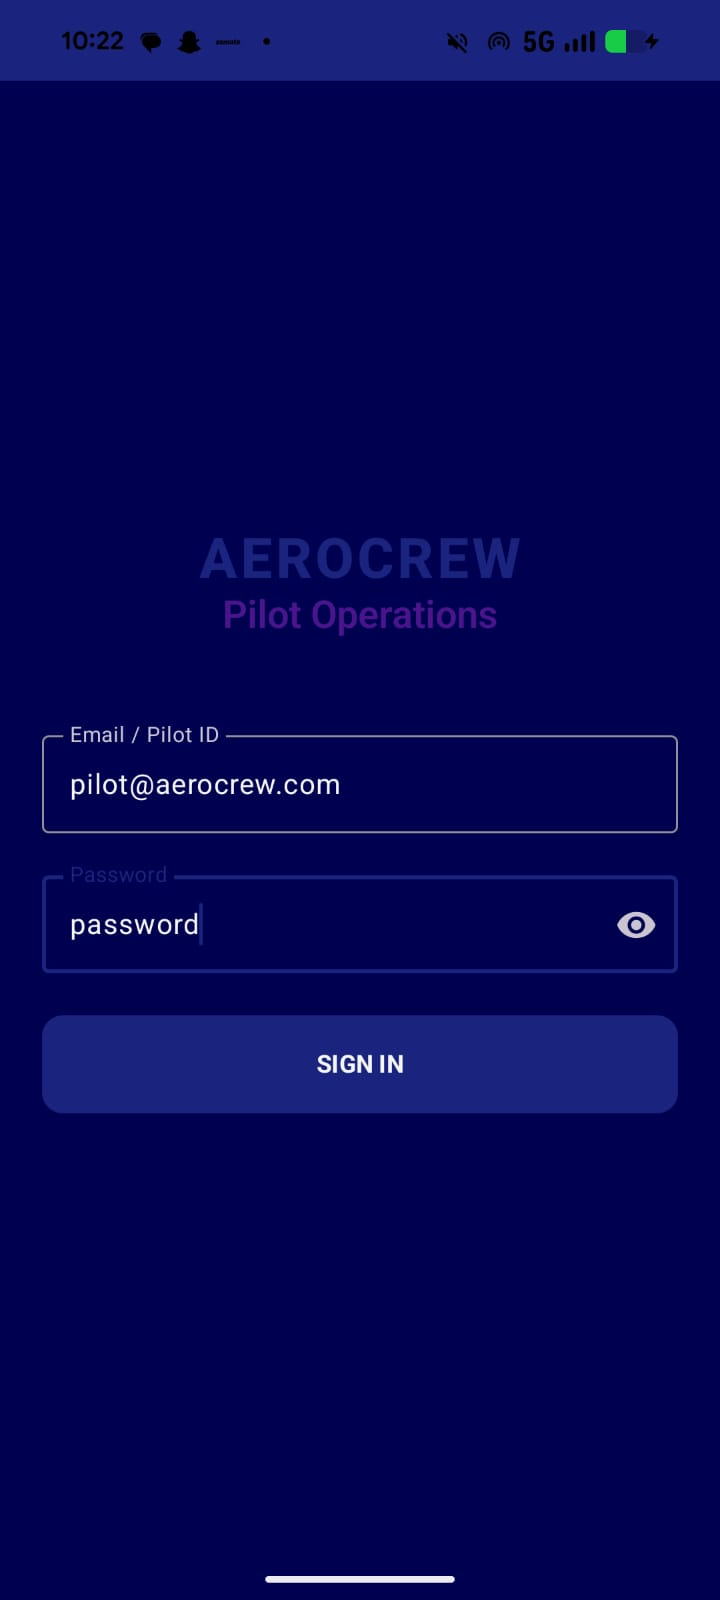
\includegraphics[width=\textwidth]{Authentication.jpeg}
    \captionof{figure}{Pilot Authentication Screen}
    \label{fig:android_authentication}
\end{minipage}
\end{figure}

\subsubsection{Pilot Dashboard and Flight Management}

After successful authentication, the pilot is presented with a dashboard containing
readiness status, today's flight information, and active operational alerts. The Flights
screen provides a consolidated view of assigned flights, including flight number, route,
departure and arrival times, aircraft type, and operational status.

\begin{figure}[H]
\centering
\begin{minipage}[t]{0.43\textwidth}
    \centering
    \includegraphics[width=\textwidth]{dashboard.jpeg}
    \captionof{figure}{Pilot Dashboard}
    \label{fig:android_dashboard}
\end{minipage}
\hfill
\begin{minipage}[t]{0.43\textwidth}
    \centering
    \includegraphics[width=\textwidth]{flight screen.jpeg}
    \captionof{figure}{My Flights Screen}
    \label{fig:android_flights}
\end{minipage}
\end{figure}

\subsubsection{Operational Alerts and Crew Recovery}

The Android application provides a dedicated alerts screen through which pilots can view
active recovery requests and other operational advisories. A crew recovery alert contains
the affected flight, route, scheduled time, and response deadline.

\begin{figure}[H]
\centering
\begin{minipage}[t]{0.43\textwidth}
    \centering
    \includegraphics[width=\textwidth]{operational alerts.jpeg}
    \captionof{figure}{Operational Alerts Screen}
    \label{fig:android_operational_alerts}
\end{minipage}
\hfill
\begin{minipage}[t]{0.43\textwidth}
    \centering
    \includegraphics[width=\textwidth]{alert details.jpeg}
    \captionof{figure}{Crew Recovery Alert Details}
    \label{fig:android_alert_details}
\end{minipage}
\end{figure}

The alert details screen allows the pilot to confirm availability or indicate
unavailability for the requested recovery operation. This response supports the
controller's crew recovery workflow and enables the pilot to participate directly in
time-sensitive operational decisions.

\subsubsection{Pilot Profile}

The Pilot Profile screen provides essential account and operational information, including
pilot ID, email address, base airport, license information, and current availability status.
The screen also provides a logout option for ending the current session.

\begin{figure}[H]
\centering
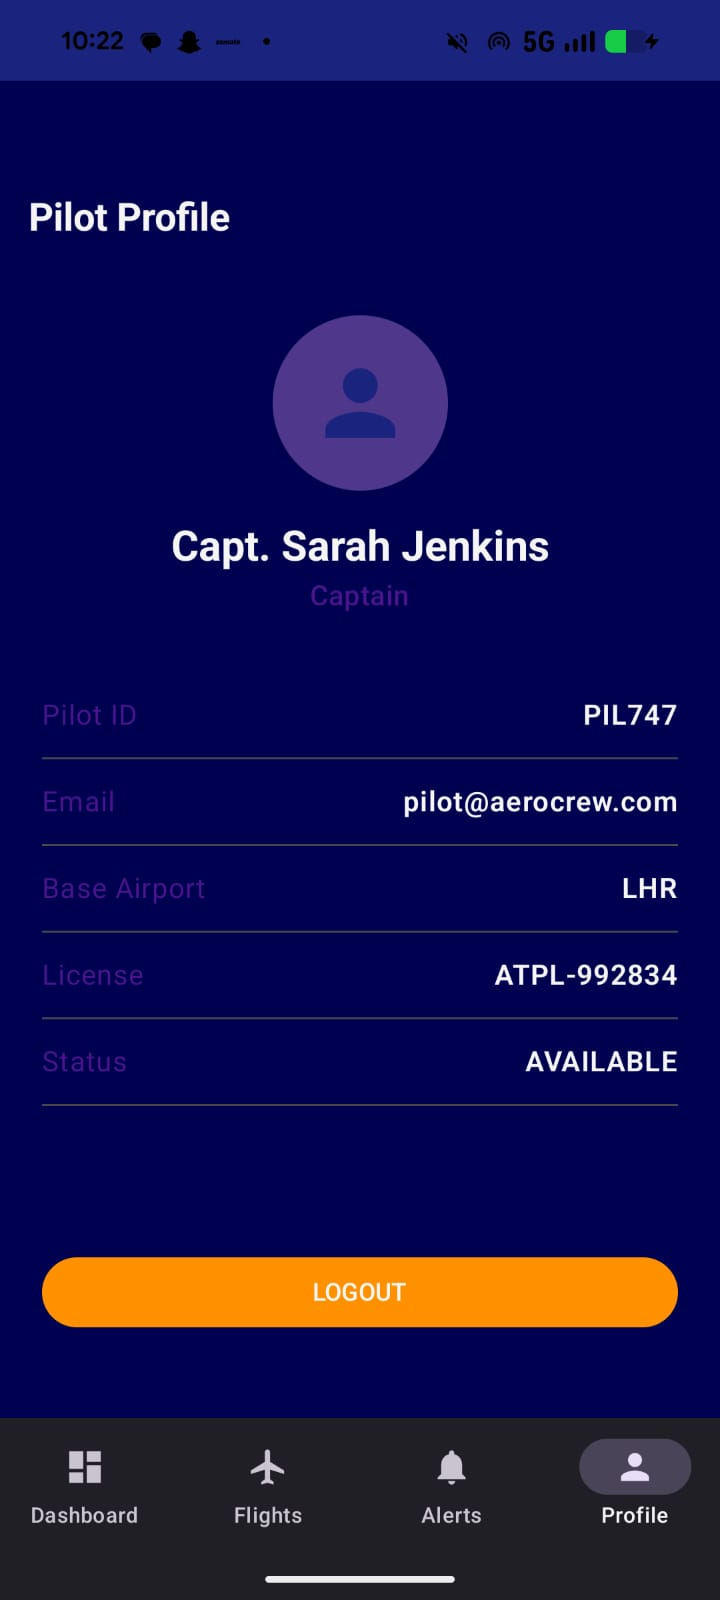
\includegraphics[width=0.43\textwidth]{Profile screen.jpeg}
\caption{Pilot Profile Screen}
\label{fig:android_profile}
\end{figure}

Overall, the integrated Android application extends AeroCrew AI beyond the Operations
Control Center by providing pilots with direct access to flight information and operational
notifications. The web and mobile components together support synchronized communication
between controllers and pilots and strengthen the human-in-the-loop crew recovery process.

%%%%%%%%%%%%%%%%%%%%%%%%%%%%%%%%%%%%%
% CHAPTER 5
%%%%%%%%%%%%%%%%%%%%%%%%%%%%%%%%%%%%%

\chapter{TESTING}

This chapter presents the testing strategy adopted to verify that AeroCrew AI meets its functional and non-functional requirements. It describes the test cases designed for key scenarios, the testing approaches followed, and the results obtained.

\section{TEST CASES}

Test cases were designed for each major functional scenario identified in the system. Table 5.1 presents the test cases defined for validating the login functionality, and Table 5.2 presents the test cases defined for validating the crew recovery recommendation functionality.

\begin{table}[H]
\centering
\caption{Test Cases -- Login Functionality}
\begin{tabular}{|p{1.5cm}|p{5cm}|p{4cm}|p{4cm}|}
\hline
\textbf{TC ID} & \textbf{Test Scenario} & \textbf{Expected Result} & \textbf{Actual Result}\\
\hline

TC01 &
Login with correct username and password &
User is authenticated and redirected to the dashboard &
As Expected\\
\hline

TC02 &
Login with an incorrect password &
System displays an ``Invalid Credentials'' error and denies access &
As Expected\\
\hline

TC03 &
Login with an incorrect username &
System displays an ``Invalid Credentials'' error and denies access &
As Expected\\
\hline

\end{tabular}
\end{table}

\begin{table}[H]
\centering
\caption{Test Cases -- Crew Recovery Recommendation}
\begin{tabular}{|p{1.5cm}|p{5cm}|p{4cm}|p{4cm}|}
\hline
\textbf{TC ID} & \textbf{Test Scenario} & \textbf{Expected Result} & \textbf{Actual Result}\\
\hline

TC04 &
Generate recommendations when eligible standby pilots exist &
System returns a ranked list of eligible pilots &
As Expected\\
\hline

TC05 &
Generate recommendations when no pilot satisfies FDTL rest requirements &
System returns an empty recommendation list with an appropriate message &
As Expected\\
\hline

TC06 &
Generate recommendations with an invalid recovery case ID &
System returns a ``Case Not Found'' error &
As Expected\\
\hline

\end{tabular}
\end{table}

Each test case verifies a specific condition of the corresponding functional scenario. For example, the login scenario requires validating a successful login as well as the two possible failure conditions (incorrect password and incorrect username), ensuring that both positive and negative paths of the functionality are covered.

\section{TESTING APPROACHES}

AeroCrew AI was tested using a combination of the following approaches to ensure correctness at both the component and system level.

\subsection{Unit Testing}

Unit testing was performed on individual components of the system in isolation, primarily targeting the service layer of the Spring Boot backend, including the compliance validation logic and the candidate ranking engine. JUnit and Mockito were used to write and execute unit tests, with mock repositories used to isolate business logic from the database layer.

\subsection{Integration Testing}

Integration testing was performed to verify that different modules of the system function correctly when combined -- for example, verifying that a disruption reported through the API correctly triggers recovery case creation, compliance validation, and candidate ranking in sequence. Integration tests were executed against a test PostgreSQL database using Spring Boot's test framework, and REST endpoints were verified using tools such as Postman and automated integration test suites.

\section{TEST REPORTS}

Table 5.3 summarizes the results obtained from executing the defined test cases with different sample inputs, demonstrating that the system produces the expected output under varying conditions.

\begin{table}[H]
\centering
\caption{Sample Test Report}
\begin{tabular}{|p{1.5cm}|p{5cm}|p{4cm}|p{2cm}|}
\hline
\textbf{TC ID} & \textbf{Sample Input} & \textbf{Observed Output} & \textbf{Status}\\
\hline

TC01 &
Username: \texttt{ops\_controller}, Password: \texttt{Correct@123} &
Dashboard loaded successfully &
Pass\\
\hline

TC02 &
Username: \texttt{ops\_controller}, Password: \texttt{Wrong@000} &
``Invalid Credentials'' error displayed &
Pass\\
\hline

TC04 &
Recovery Case ID: 105 (3 eligible standby pilots) &
Ranked list of 3 pilots returned &
Pass\\
\hline

TC05 &
Recovery Case ID: 106 (no pilot meets rest requirement) &
Empty recommendation list with message &
Pass\\
\hline

TC06 &
Recovery Case ID: 999 (non-existent) &
``Case Not Found'' error returned &
Pass\\
\hline

\end{tabular}
\end{table}

The results obtained confirm that AeroCrew AI performs as expected across normal, boundary, and failure conditions, validating both the functional correctness of individual modules and the reliability of the integrated system.

%%%%%%%%%%%%%%%%%%%%%%%%%%%%%%%%%%%%%
% CHAPTER 6
%%%%%%%%%%%%%%%%%%%%%%%%%%%%%%%%%%%%%

\chapter{CONCLUSION}

This chapter reflects on the design and implementation challenges encountered during the development of AeroCrew AI, discusses the advantages and limitations of the proposed system, and outlines directions for future enhancement.

\section{DESIGN AND IMPLEMENTATION ISSUES}

\subsection{Design Issues}

Several challenges were encountered during the design phase of AeroCrew AI. One of the major challenges was requirements volatility, as airline crew regulations and operational parameters can change over time. Therefore, the system had to be designed with configurable compliance rules rather than relying on hard-coded logic, which required additional design iterations.

Scalability was another important challenge. Designing a system capable of supporting an increasing number of flights, pilots, and concurrent users required careful selection of a layered, stateless REST architecture along with an efficiently indexed database schema. This ensured that the system could accommodate future growth without requiring major architectural changes.

Performance also presented a significant challenge, particularly in ensuring that compliance validation and candidate ranking could be completed within a few seconds even when the number of standby pilots increased. To address this requirement, database queries needed to be optimized and unnecessary calls to external APIs had to be minimized.

Security was another key consideration during the design process. The system needed to securely differentiate between multiple user roles, including Administrator, Crew Controller, Operations Controller, OCC Manager, and Pilot. Implementing appropriate authentication and authorization mechanisms for these different roles added complexity to the access-control design.

Finally, usability was an important design challenge. The dashboard needed to provide controllers with sufficient operational information while maintaining a simple and intuitive interface. Since controllers often work under significant time pressure, several rounds of interface refinement were required to achieve an appropriate balance between information availability and ease of use.

\subsection{Implementation Issues}

Several challenges were encountered during the implementation of AeroCrew AI. One of the major challenges was maintaining a consistent operating environment across the web, backend, and Android components. To minimize environment-specific issues and ensure consistency during development and testing, containerization using Docker was adopted.

Another challenge involved external API dependency. The integration of third-party weather and traffic APIs introduced dependencies on the availability and response times of external services. During testing, occasional delays or unavailability of these services affected the accuracy and consistency of travel-time estimation.

Installation and configuration also required significant attention. Setting up the PostgreSQL database, environment variables, and Firebase configuration consistently across different development machines required standardized setup scripts and supporting documentation. This helped ensure that all team members could configure and run the system using a consistent environment.

Finally, data migration and testing presented a challenge because realistic operational data was required to test pilots, flights, and disruption scenarios. Since real airline operational data was not available for the project, additional effort was required to generate suitable sample data for testing and validating the different functionalities of AeroCrew AI.



\section{ADVANTAGES AND LIMITATIONS}

\subsection{Advantages}

AeroCrew AI addresses several limitations of the existing manual crew recovery process identified in Chapter 2. The system replaces slow and manual verification of pilot eligibility with automated, rule-based compliance validation, thereby reducing the time required to make crew recovery decisions.

The system also provides a single, centralized platform instead of relying on multiple disconnected systems and spreadsheets. This improves operational visibility and allows controllers to access relevant crew, flight, and disruption information from a unified interface.

AeroCrew AI introduces objective and explainable candidate ranking, reducing dependence on individual controller judgment and improving consistency across crew recovery decisions. The system also incorporates automated travel-time estimation, a capability that was absent from the existing manual recovery process and which supports more informed crew assignment decisions.

Finally, the system improves auditability through comprehensive activity logging. Recording important operational activities supports regulatory compliance, accountability, and traceability of crew recovery decisions.

\subsection{Limitations}

Despite its benefits, the current implementation of AeroCrew AI has certain limitations. The integration with live airline reservation and crew scheduling systems has not been implemented in the current version and is instead simulated using sample operational data. As a result, the system has not yet been validated against live airline operational environments.

The travel-time estimation module depends on the accuracy and availability of third-party weather and traffic APIs. Any delay, unavailability, or inaccurate information from these external services may occasionally affect travel-time estimation and, consequently, the accuracy of operational recommendations.

Another limitation is the absence of predictive, machine-learning-based disruption forecasting. Although predictive analytics was identified as a valuable enhancement, it was not implemented due to the scope and time constraints of the project. Similarly, load testing was performed using a limited dataset, and the system's performance under very large-scale, nationwide airline operations has not yet been fully validated.

During the review and demonstration of the system, it was also suggested that further customization of dashboard views for different user roles could improve usability. This enhancement has therefore been identified as a future improvement rather than being implemented in the current version.

\section{FUTURE SCOPE OF THE PROJECT}

Several areas of investigation and enhancement were identified during the development of AeroCrew AI that could be pursued in future iterations of the project. One important area is predictive disruption analytics, which would involve incorporating machine learning models trained on historical operational data to proactively predict potential crew disruptions before they occur. This could help airline controllers take preventive measures and improve operational preparedness.

Another potential enhancement is the integration with airline reservation systems. The platform could be extended to directly integrate with live airline reservation, crew scheduling, and flight planning systems, enabling fully automated synchronization of operational data. The system could also be enhanced to provide multi-airline and multi-base support, allowing multiple airline operators and crew bases to be managed within a single deployment.

The Android mobile application could also be expanded with advanced features such as offline support, in-app communication between controllers and pilots, and additional self-service functionalities for pilots. Another important area for future development is automated regulatory updates. A configurable rules engine could be developed to allow DGCA and other regulatory compliance rules to be updated without requiring changes to the underlying application code.

Due to time constraints, several of these enhancements, particularly predictive analytics and full integration with external airline systems, could not be completed within the scope of the current project. These features are therefore recommended as important directions for future development of AeroCrew AI.

\end{document}